

%%
%% forked from https://gits-15.sys.kth.se/giampi/kthlatex kthlatex-0.2rc4 on 2020-02-13
%% expanded upon by Gerald Q. Maguire Jr.
%% This template has been adapted by Anders Sjögren to the University
%% Engineering Program in Computer Science at KTH ICT. Adaptation is the
%% translation of English headings into Swedish as the addition of Swedish
%% text. Original body text is deliberately left in English.

%% Conventions for todo notes:
% \todo[inline]{Comments/directions/... in English}
% \todo[inline, backgroundcolor=kth-lightblue]{Text på svenska}
% \todo[inline, backgroundcolor=kth-lightgreen]{English descriptions about formatting}

%% The template is designed to handle a thesis in English or Swedish
% set the default language to english or swedish by passing an option to the documentclass - this handles the inside tile page
% To optimize for digital output (this changes the color palette add the option: digitaloutput
% To use bibtex or biblatex - include one of these as an option
\documentclass[oneside, english, bibtex]{kththesis}
%\documentclass[oneside, swedish, biblatex]{kththesis}
\usepackage[activate={true,nocompatibility},final,tracking=true,kerning=true,spacing=true,factor=1100,stretch=10,shrink=10]{microtype}
\usepackage{tikz}
\usepackage{float}

% \usepackage[style=numeric,sorting=none,backend=biber]{biblatex}
\ifbiblatex
    %\usepackage[language=english,bibstyle=authoryear,citestyle=authoryear, maxbibnames=99]{biblatex}
     \usepackage[bibstyle=authoryear,citestyle=authoryear, maxbibnames=99,language=english]{biblatex}
    \addbibresource{references.bib}
\else
    % The line(s) below are for BibTeX
    \bibliographystyle{bibstyle/myIEEEtran}
    %\bibliographystyle{apalike}
\fi


% include a variety of packages that are useful
%%%%%%%%%%%%%%%%%%%%%%%%%%%%%% Packages %%%%%%%%%%%%%%%%%%%%%%%%%%%%%%
%% The following are needed for generating the DiVA page(s)
\usepackage{scontents}              %% Needed to save lang, abstract, and keywords
\usepackage{pgffor}                 %% includes the foreach loop

%% Basic packages

%% Links
\usepackage{url}                %% Support for breaking URLs

%% Colorize
%\usepackage{color}
\PassOptionsToPackage{dvipsnames, svgnames}{xcolor}
\usepackage{xcolor}

\usepackage[normalem]{ulem}
\usepackage{soul}
\usepackage{xspace}
\usepackage{braket}

% to support units and decimal aligned columns in tables
% the option loads the binary prefixes
\usepackage[binary-units=true, locale=US]{siunitx}

\usepackage{balance}
\usepackage{stmaryrd}
\usepackage{booktabs}
\usepackage{graphicx}	        %% Support for images
\usepackage{multirow}	        %% Support for multirow columns in tables
\usepackage{tabularx}		    %% For simple table stretching
\usepackage{mathtools}
\usepackage{algorithm} 
\usepackage{algorithmic}  
\usepackage{amsmath}
\usepackage[linesnumbered,ruled,vlined,algo2e]{algorithm2e}
% can't use both algpseudocode and algorithmic packages
%\usepackage[noend]{algpseudocode}
%\usepackage{subfig}  %% cannot use both subcaption and subfig packages
\usepackage{optidef}
\usepackage{float}		        %% Support for more flexible floating box positioning
\usepackage{pifont}

%% some additional useful packages
% to enable rotated figures
\usepackage{rotating}	    	%% For text rotating
\usepackage{array}		        %% For table wrapping
\usepackage{mdwlist}            %% various list-related commands
\usepackage{setspace}           %% For fine-grained control over line spacing


\usepackage{enumitem}           %% to allow changes to the margins of descriptions


%% If you are going to include source code (or code snippets)
\usepackage{listings}		    %% For source code listing
%%\usepackage[cache=false]{minted} %% For source code highlighting
%%\usemintedstyle{borland}

\usepackage{bytefield}          %% For packet drawings


\setlength {\marginparwidth }{2cm} %leave some extra space for todo notes
\usepackage{todonotes}
\usepackage{notoccite} % do not number captions based on their appearance in the TOC


% Footnotes
\usepackage{perpage}
\usepackage[perpage,para,symbol]{footmisc} %% use symbols to ``number'' footnotes and reset which symbol is used first on each page


%% Various useful packages
%%----------------------------------------------------------------------------
%%   pcap2tex stuff
%%----------------------------------------------------------------------------
\usepackage{tikz}
\usetikzlibrary{arrows,decorations.pathmorphing,backgrounds,fit,positioning,calc,shapes}
\usepackage{pgfmath}	% --math engine
\newcommand\bmmax{2}
\usepackage{bm} % bold math


%% Managing titles
% \usepackage[outermarks]{titlesec}
%%%%%%%%%%%%%%%%%%%%%%%%%%%%%%%%%%%%%%%%%%%%%%%%%%%%%%%%%%%%%%%%%%%%%%
%\captionsetup[subfloat]{listofformat=parens}

% to include PDF pages
%\usepackage{pdfpages}


\usepackage{csquotes}               %% Recommended by biblatex
% to provide a float barrier use:
\usepackage{placeins}

\usepackage{comment}  %% Provides a comment environment




%%% Local Variables:
%%% mode: latex
%%% TeX-master: t
%%% End:
% KTH colors for LaTeX documents
%
% Started from kthcolors by:
% Riccardo Sven Risuleo
% 2016-09-06 11:05:40
%
% from https://github.com/KTH-AC/kthcolors
%
% Adapted using the colors from "Graphic Profile Manual KTH" version 180604
% (i.e.. 2018-06-04) 
% see https://intra.kth.se/en/administration/kommunikation/grafiskprofil/kth-s-grafiska-profil-1.844676
% 
% G. Q. Maguire Jr.
% 2021-07-05
%

%\NeedsTexFormat{LaTeX2e}[1994/06/01]
%\ProvidesPackage{kthcolors}[2021/07/85 v3 Latex package with official KTH colors]

\RequirePackage{xcolor}
%% Primary colors
%% As of the new manual, there is only 1 primary color; but with three 
\definecolor{kth-blue}{RGB/cmyk}{25,84,166/0.849,0.494,0,0.349}
\colorlet{kth-blue80}{kth-blue!80!}
\colorlet{kth-blue40}{kth-blue!40!}

% these are no longer used as of 2018-06-04
%\definecolor{kth-red}{RGB/cmyk}{157,16,45/0,0.898,0.713,0.384}
%\definecolor{kth-green}{RGB/cmyk}{98,146,46/0.329,0,0.685,0.427}

%% Secondary colors
\definecolor{kth-lightblue}{RGB/cmyk}{36,160,216/0.833,0.259,0,0.153}
\colorlet{kth-lightblue80}{kth-lightblue!80!}
\colorlet{kth-lightblue40}{kth-lightblue!40!}

%\definecolor{kth-lightred}{RGB/cmyk}{228,54,62/0,0.763,0.728,0.106}
\definecolor{kth-lightred}{RGB}{216,84,151}
\colorlet{kth-lightred80}{kth-lightred!80!}
\colorlet{kth-lightred40}{kth-lightred!40!}

\definecolor{kth-lightgreen}{RGB/cmyk}{176,201,43/0.124,0,0.786,0.212} % olive
\colorlet{kth-lightgreen80}{kth-lightgreen!80!}
\colorlet{kth-lightgreen40}{kth-lightgreen!40!}

% Cool Gray 9C
%\definecolor{kth-coolgray}{RGB}{101,101,108}

% Cool Gray 10 suggested by Martin Krzywinski (see http://mkweb.bcgsc.ca/colorblind) 
\definecolor{kth-coolgray}{RGB}{99,102,106}
\colorlet{kth-coolgray80}{kth-coolgray!80!}
\colorlet{kth-coolgray40}{kth-coolgray!40!}

% Tertiary colors (yet more colors)
% All of these are no longer used
%\definecolor{kth-pink}{RGB/cmyk}{216,84,151/10,0.611,0.301,0.153}
%\definecolor{kth-yellow}{RGB/cmyk}{250,185,25/0,0.26,0.9,0.0196}
%\definecolor{kth-darkgray}{RGB/cmyk}{101,101,108/0.0648,0.0648,0,0.576}
%\definecolor{kth-middlegray}{RGB/cmyk}{189,188,188/0,0.00529,0.00529,0.259}
%\definecolor{kth-lightgray}{RGB/cmyk}{227,229,227/0.00873,0,0.00873,0.102}

%\DeclareOption{gray}{\colorlet{gray}{kth-darkgray}}

% These versions are designed to meet accessability requirements for digital media
% Note that the palette is more limited than for the print version of the colors
\ifdigitaloutput
    % primary color
    \definecolor{kth-blue}{HTML}{1954A6} % Deep sea
    \definecolor{kth-blue80}{HTML}{5E87C0}

    % Secondary colors
    \definecolor{kth-lightblue}{HTML}{2191C4} % Stratosphere
    \definecolor{kth-lightred}{HTML}{D02F80} % Fluorescence
    \definecolor{kth-lightred80}{HTML}{D95599}
    \definecolor{kth-lightgreen}{HTML}{62922E} % Front-lawn
    \definecolor{kth-coolgray}{HTML}{65656C} % Office
    \definecolor{kth-coolgray80}{HTML}{848489}
\fi



%\glsdisablehyper
%\makeglossaries
%\makenoidxglossaries
%%%% Local Variables:
%%% mode: latex
%%% TeX-master: t
%%% End:

% The form of the entries in this file is \newacronym{label}{acronym}{phrase}
%                                      or \newacronym[options]{label}{acronym}{phrase}
% see "User Manual for glossaries.sty" for the  details about the options, one example is shown below
% note the specification of the long form plural in the line below
%\newacronym[longplural={Debugging Information Entities}]{DIE}{DIE}{Debugging Information Entity}
%
% The following example also uses options
%\newacronym[plural={OSes}, firstplural={operating systems (OSes)}]{OS}{OS}{operating system}

% note the use of a non-breaking dash in long text for the following acronym
%\newacronym{IQL}{IQL}{Independent Q‑Learning}

%\newacronym{LAN}{LAN}{Local Area Network}
% note the use of a non-breaking dash in the following acronym
%\newacronym{WiFi}{Wi-Fi}{Wireless Fidelity}

%\newacronym{WLAN}{WLAN}{Wireless Local Area Network}
%\newacronym{UN}{UN}{United Nations}
%\newacronym{SDG}{SDG}{Sustainable Development Goal}

\newacronym{ANN}{ANN}{Artificial Neural Network}
\newacronym{BERT}{BERT}{Bidirectional Encoder Representations from Transformers}
\newacronym{BoW}{BoW}{Bag of Words}

\newacronym{COCO}{COCO}{Common Objects in Context}
\newacronym{CBOW}{CBOW}{Continuous Bag of Words}
\newacronym{CNN}{CNN}{Convolutional Neural Network}

\newacronym{DN}{DN}{Dagens Nyheter}
\newacronym{DNN}{DNN}{Deep Neural Network}

\newacronym{FN}{FN}{False Negative}
\newacronym{FP}{FP}{False Positive}
\newacronym{FPN}{FPN}{Feature Pyramid Network}
\newacronym{FCNN}{FCN}{Fully Convolutional (Neural) Network}

\newacronym{GloVe}{GloVe}{Global Vectors}
\newacronym{GPU}{GPU}{Graphical Processing Unit}

\newacronym{IoU}{IoU}{Intersection over Union}

\newacronym{mAP}{mAP}{mean Average Precision}
\newacronym{mIoU}{mIoU}{mean Interesection over Union}
\newacronym{MLP}{MLP}{Multilayer Perceptron}
\newacronym{NLP}{NLP}{Natural Language Processing}

\newacronym{OCR}{OCR}{Optical Character Recognition}

\newacronym{RGB}{RGB}{Red Green Blue}
\newacronym{R-CNN}{R-CNN}{Region Based Convolutional Neural Network}
\newacronym{RoI}{RoI}{Region of Interest}
\newacronym{ResNet}{ResNet}{Residual Neural Network}
\newacronym{ReLU}{ReLU}{Rectified Linear Unit}
\newacronym{RPN}{RPN}{Region Proposal Network}
\newacronym{RLSA}{RLSA}{Run-Length Smoothing Algorithm}


\newacronym{SBERT}{SBERT}{Sentence-BERT}
\newacronym{SvD}{SVD}{Svenska Dagbladet}

\newacronym{TF}{TF}{Term Frequency}
\newacronym{TF-IDF}{TF-IDF}{Term Frequency-Inverse Document Frequency}
\newacronym{TN}{TN}{True Negative}
\newacronym{TP}{TP}{True Positive}
                %load the acronyms file

\makeatletter
\newcommand{\DeclareLatinAbbrev}[2]{%
  \DeclareRobustCommand{#1}{%
    \@ifnextchar{.}{\textit{#2}}{%
      \@ifnextchar{,}{\textit{#2.}}{%
        \@ifnextchar{!}{\textit{#2.}}{%
          \@ifnextchar{?}{\textit{#2.}}{%
            \@ifnextchar{)}{\textit{#2.}}{%
              {\textit{#2.,\ }}}}}}}}%
}
\makeatother
\DeclareLatinAbbrev{\eg}{e.g}
\DeclareLatinAbbrev{\Eg}{E.g}
\DeclareLatinAbbrev{\ie}{i.e}
\DeclareLatinAbbrev{\Ie}{I.e}
\DeclareLatinAbbrev{\etc}{etc}
\DeclareLatinAbbrev{\etal}{et~al}

\def\first {$(i)$\xspace}
\def\second{$(ii)$\xspace}
\def\third {$(iii)$\xspace}
\def\fourth{$(iv)$\xspace}
\def\fifth {$(v)$\xspace}
\def\sixth {$(vi)$\xspace}
\def\seventh{$(vii)$\xspace}
\def\eighth{$(viii)$\xspace}

%%% custom definitions
%% Coloring the links!
\newcommand\myshade{75} % Usage: red!\myshade!black

\definecolor{ForestGreen} {RGB}{34,  139,  34}
\definecolor{HeraldRed2}   {rgb}{0.81, 0.12, 0.15}

\newcommand{\refscolor} {blue}
\newcommand{\linkscolor}{HeraldRed2}
\newcommand{\urlscolor} {ForestGreen}

%% Some definitions of used colors
%\definecolor{darkblue}{rgb}{0.0,0.0,0.3} %% define a color called darkblue
%\definecolor{darkred}{rgb}{0.4,0.0,0.0}
%\definecolor{red}{rgb}{0.7,0.0,0.0}
%\definecolor{lightgrey}{rgb}{0.8,0.8,0.8} 
%\definecolor{grey}{rgb}{0.6,0.6,0.6}
%\definecolor{darkgrey}{rgb}{0.4,0.4,0.4}
%\definecolor{aqua}{rgb}{0.0, 1.0, 1.0}

% For runin headings
\newcommand{\smartparagraph}[1]{\vspace{.05in}\noindent\textbf{#1}}

%% Table of Contents (ToC) depth 
\setcounter{secnumdepth}{4} % how many sectioning levels to assign numbers to
\setcounter{tocdepth}{4}    % how many sectioning levels to show in ToC

%% Limit hyphenation
\hyphenpenalty=9000
\tolerance=5000
% Reduce hyphenation as much as possible:
%\hyphenpenalty=15000
%\tolerance=1000

% For notes by the authors to themselves
\newcommand*{\todoinline}[1]{\textcolor{red}{TODO: #1}}
  % load some additional definitions to make writing more consistent

% The following is needed in conjunction with generating the DiVA data with abstracts and keywords using the scontents package and a modified listings environment
%\usepackage{listings}   %  already included
\ExplSyntaxOn
\newcommand\typestoredx[2]{\expandafter\__scontents_typestored_internal:nn\expandafter{#1} {#2}}
\ExplSyntaxOff
\makeatletter
\let\verbatimsc\@undefined
\let\endverbatimsc\@undefined
\lst@AddToHook{Init}{\hyphenpenalty=50\relax}
\makeatother


\lstnewenvironment{verbatimsc}
    {
    \lstset{%
        basicstyle=\ttfamily\tiny,
        backgroundcolor=\color{white},
        %basicstyle=\tiny,
        %columns=fullflexible,
        columns=[l]fixed,
        language=[LaTeX]TeX,
        %numbers=left,
        %numberstyle=\tiny\color{gray},
        keywordstyle=\color{red},
        breaklines=true,                 % sets automatic line breaking
        breakatwhitespace=true,          % sets if automatic breaks should only happen at whitespace
        %keepspaces=false,
        breakindent=0em,
        %fancyvrb=true,
        frame=none,                     % turn off any box
        postbreak={}                    % turn off any hook arrow for continuation lines
    }
}{}



%% definition of new command for bytefield package
\newcommand{\colorbitbox}[3]{%
	\rlap{\bitbox{#2}{\color{#1}\rule{\width}{\height}}}%
	\bitbox{#2}{#3}}

%% Acronyms
% note that nonumberlist - removes the cross references to the pages where the acronym appears
% note that nomain - does not produce a main glossary, this only acronyms will be in the glossary
% note that nopostdot - will present there being a period at the end of each entry
\usepackage[acronym, section=section, nonumberlist, nomain, nopostdot]{glossaries}
\usepackage[automake]{glossaries-extra}
\ifinswedish
    %\usepackage{glossaries-swedish}
\fi

% Because backref is not compatible with biblatex
\ifbiblatex
    \usepackage[plainpages=false]{hyperref}
\else
    \usepackage[
    backref=page,
    pagebackref=false,
    plainpages=false,
                            % PDF related options
    unicode=true,           % Unicode encoded PDF strings
    bookmarks=true,         % generate bookmarks in PDF files
    bookmarksopen=false,    % Do not automatically open the bookmarks in the PDF reading program
    pdfpagemode=UseNone,    % None, UseOutlines, UseThumbs, or FullScreen
    ]{hyperref}
    \usepackage{backref}
    %
    % Customize list of backreferences.
    % From https://tex.stackexchange.com/a/183735/1340
    \renewcommand*{\backref}[1]{}
    \renewcommand*{\backrefalt}[4]{%
    \ifcase #1%
          \or [Page~#2.]%
          \else [Pages~#2.]%
    \fi%
    }
\fi
\usepackage[all]{hypcap}	%% prevents an issue related to hyperref and caption linking


% packages that have to be included after hyperref
\usepackage{doi}
\usepackage{cleveref}           %% Replace Section with a symbol


%\glsdisablehyper
\makeglossaries
%%% Local Variables:
%%% mode: latex
%%% TeX-master: t
%%% End:

% The form of the entries in this file is \newacronym{label}{acronym}{phrase}
%                                      or \newacronym[options]{label}{acronym}{phrase}
% see "User Manual for glossaries.sty" for the  details about the options, one example is shown below
% note the specification of the long form plural in the line below
%\newacronym[longplural={Debugging Information Entities}]{DIE}{DIE}{Debugging Information Entity}
%
% The following example also uses options
%\newacronym[plural={OSes}, firstplural={operating systems (OSes)}]{OS}{OS}{operating system}

% note the use of a non-breaking dash in long text for the following acronym
%\newacronym{IQL}{IQL}{Independent Q‑Learning}

%\newacronym{LAN}{LAN}{Local Area Network}
% note the use of a non-breaking dash in the following acronym
%\newacronym{WiFi}{Wi-Fi}{Wireless Fidelity}

%\newacronym{WLAN}{WLAN}{Wireless Local Area Network}
%\newacronym{UN}{UN}{United Nations}
%\newacronym{SDG}{SDG}{Sustainable Development Goal}

\newacronym{ANN}{ANN}{Artificial Neural Network}
\newacronym{BERT}{BERT}{Bidirectional Encoder Representations from Transformers}
\newacronym{BoW}{BoW}{Bag of Words}

\newacronym{COCO}{COCO}{Common Objects in Context}
\newacronym{CBOW}{CBOW}{Continuous Bag of Words}
\newacronym{CNN}{CNN}{Convolutional Neural Network}

\newacronym{DN}{DN}{Dagens Nyheter}
\newacronym{DNN}{DNN}{Deep Neural Network}

\newacronym{FN}{FN}{False Negative}
\newacronym{FP}{FP}{False Positive}
\newacronym{FPN}{FPN}{Feature Pyramid Network}
\newacronym{FCNN}{FCN}{Fully Convolutional (Neural) Network}

\newacronym{GloVe}{GloVe}{Global Vectors}
\newacronym{GPU}{GPU}{Graphical Processing Unit}

\newacronym{IoU}{IoU}{Intersection over Union}

\newacronym{mAP}{mAP}{mean Average Precision}
\newacronym{mIoU}{mIoU}{mean Interesection over Union}
\newacronym{MLP}{MLP}{Multilayer Perceptron}
\newacronym{NLP}{NLP}{Natural Language Processing}

\newacronym{OCR}{OCR}{Optical Character Recognition}

\newacronym{RGB}{RGB}{Red Green Blue}
\newacronym{R-CNN}{R-CNN}{Region Based Convolutional Neural Network}
\newacronym{RoI}{RoI}{Region of Interest}
\newacronym{ResNet}{ResNet}{Residual Neural Network}
\newacronym{ReLU}{ReLU}{Rectified Linear Unit}
\newacronym{RPN}{RPN}{Region Proposal Network}
\newacronym{RLSA}{RLSA}{Run-Length Smoothing Algorithm}


\newacronym{SBERT}{SBERT}{Sentence-BERT}
\newacronym{SvD}{SVD}{Svenska Dagbladet}

\newacronym{TF}{TF}{Term Frequency}
\newacronym{TF-IDF}{TF-IDF}{Term Frequency-Inverse Document Frequency}
\newacronym{TN}{TN}{True Negative}
\newacronym{TP}{TP}{True Positive}
                %load the acronyms file

%% Information for inside title page
\title{News article segmentation using multimodal input}
\subtitle{Using Mask R-CNN and sentence transformers}

% give the alternative title - i.e., if the thesis is in English, then give a Swedish title
\alttitle{Artikelsegmentering med multimodala artificiella neuronnätverk}
\altsubtitle{Med hjälp av Mask R-CNN och sentence transformers}
% alternative, if the thesis is in Swedish, then give an English title
%\alttitle{This is the English translation of the title}
%\altsubtitle{This is the English translation of the subtitle}

\authorsLastname{Henning}
\authorsFirstname{Gustav}
\email{ghenning@kth.se}
\kthid{ghenning}
% If the student has an ORCiD - add it here
%\orcid{0000-0002-00001-1234}
\authorsSchool{\schoolAcronym{CDATE}}

\supervisorAsLastname{Nyberg}
\supervisorAsFirstname{Jakob}
\supervisorAsEmail{jaknyb@kth.se}
% If the supervisor is from within KTH add their KTHID, School and Department info
\supervisorAsKTHID{jaknyb}
\supervisorAsSchool{\schoolAcronym{EECS}}
\supervisorAsDepartment{Computer Science}

\examinersLastname{Aristides}
\examinersFirstname{Gionis}
\examinersEmail{argioni@kth.se}
% If the examiner is from within KTH add their KTHID, School and Department info
\examinersKTHID{argioni}
\examinersSchool{\schoolAcronym{EECS}}
\examinersDepartment{Theoretical Computer Science}
% other for a examiner outside of KTH add their organization info
%\examinersOrganization{Timbuktu University, Department of Pseudoscience}


\hostorganization{National Library of Sweden, Kungliga Biblioteket}   % if there was a host organization


\date{\today}


% For a CDATE student the following are likely values:
\programcode{CDATE}
\courseCycle{2}
\courseCode{DA231X}
\courseCredits{30.0}
\examName{Degree of Master of Science in Engineering}
\subjectArea{Computer Science and Engineering}


%%%%% For the oral presentation
%% Add this information once your examiner has scheduled your oral presentation
\presentationDateAndTimeISO{2021-03-15 13:00}
\presentationLanguage{eng}
\presentationRoom{via Zoom https://kth-se.zoom.us/j/ddddddddddd}
\presentationAddress{Isafjordsgatan 22 (Kistagången 16)}
\presentationCity{Stockholm}

% When there are multiple opponents, separate their names with '\&'
% Opponent's information
\opponentsNames{A. B. Normal \& A. X. E. Normalè}

%%%%% for DiVA's National Subject Category information
%%% Enter one or more 3 or 5 digit codes
%%% See https://www.scb.se/contentassets/3a12f556522d4bdc887c4838a37c7ec7/standard-for-svensk-indelning--av-forskningsamnen-2011-uppdaterad-aug-2016.pdf
%%% See https://www.scb.se/contentassets/10054f2ef27c437884e8cde0d38b9cc4/oversattningsnyckel-forskningsamnen.pdf
%%%%
%%%% Some examples of these codes are shown below:
% 102 Data- och informationsvetenskap (Datateknik)    Computer and Information Sciences
% 10201 Datavetenskap (datalogi) Computer Sciences
% 10202 Systemvetenskap, informationssystem och informatik (samhällsvetenskaplig inriktning under 50804)
% Information Systems (Social aspects to be 50804)
% 10203 Bioinformatik (beräkningsbiologi) (tillämpningar under 10610)
% Bioinformatics (Computational Biology) (applications to be 10610)
% 10204 Människa-datorinteraktion (interaktionsdesign) (Samhällsvetenskapliga aspekter under 50803) Human Computer Interaction (Social aspects to be 50803)
% 10205 Programvaruteknik Software Engineering
% 10206 Datorteknik Computer Engineering
% 10207 Datorseende och robotik (autonoma system) Computer Vision and Robotics (Autonomous Systems)
% 10208 Språkteknologi (språkvetenskaplig databehandling) Language Technology (Computational Linguistics)
% 10209 Medieteknik Media and Communication Technology
% 10299 Annan data- och informationsvetenskap Other Computer and Information Science
%%%
% 202 Elektroteknik och elektronik Electrical Engineering, Electronic Engineering, Information Engineering
% 20201 Robotteknik och automation Robotics
% 20202 Reglerteknik Control Engineering
% 20203 Kommunikationssystem Communication Systems
% 20204 Telekommunikation Telecommunications
% 20205 Signalbehandling Signal Processing
% 20206 Datorsystem Computer Systems
% 20207 Inbäddad systemteknik Embedded Systems
% 20299 Annan elektroteknik och elektronik Other Electrical Engineering, Electronic Engineering, Information Engineering
%% Example for a thesis in Computer Science and Computer Systems
\nationalsubjectcategories{10201, 10207}

% Enter the English and Swedish keywords here for use in the PDF meta data _and_ for later use
% following the respective abstract.
% Try to put the words in the same order in both languages to facilitate matching. For example:
\EnglishKeywords{Historical newspapers, Image segmentation, Multimodal learning, Deep learning, Digital humanities, Mask R-CNN}
\SwedishKeywords{Historiska tidningar, Bildsegmentering, Multimodal inlärning, Djupinlärning, Digital humaniora, Mask R-CNN}

% Put the title, author, and keyword information into the PDF meta information TODO
% This file contains the LaTeX to add information to the PDF file (specifically, author(s), title(s), and keywords
% It uses the hyperref package and should be be included before the \begin{document}
%
% I want to acknowledge the inspiration of Karl Voit's template for TU Graz that inspired me to add the PDF document information
% For more information about his template see https://github.com/novoid/LaTeX-KOMA-template
% Note that this template does not use anything from his template other than the names of the information for the PDF meta fields, i.e., mytitle, myauthor, and mykeywords together with the idea of defining the corresponding newcommand to set the relevant hyperref parameters.

\makeatletter
\ifx\@subtitle\@empty
    \newcommand{\mytitle}{\@title}
\else
    \newcommand{\mytitle}{\@title: \@subtitle}
\fi
\makeatother

\hypersetup{
     pdftitle={\mytitle}        % Title field
}

\makeatletter
\ifx\@secondAuthorsLastname\@empty
    \newcommand{\myauthor}{\@authorsFirstname\space\@authorsLastname} 
\else
    \ifinswedish
    \newcommand{\myauthor}{\@authorsFirstname\space\@authorsLastname\space\relax och\space\@secondAuthorsFirstname \@secondAuthorsLastname}
    \else
        \newcommand{\myauthor}{\@authorsFirstname\space\@authorsLastname\space\relax and\space\@secondAuthorsFirstname \@secondAuthorsLastname}
    \fi
\fi
\makeatother

\hypersetup{
     pdfauthor={\myauthor}      % Author field
}

% Put the alternative title (and subtitle) into the PDF Subject meta
\makeatletter
\ifx\@altsubtitle\@empty\relax
    \newcommand{\myalttitle}{\@alttitle}
\else
    \newcommand{\myalttitle}{\@alttitle: \@altsubtitle}
\fi
\makeatother

\hypersetup{
     pdfsubject={\myalttitle}        % Subject field
}

\makeatletter
\ifx\@EnglishKeywords\@empty
    \ifx\@SwedishKeywords\@empty
        \newcommand{\mykeywords}{}
    \else
    \newcommand{\mykeywords}{\@SwedishKeywords}
    \fi
\else
    \ifx\@SwedishKeywords\@empty
        \newcommand{\mykeywords}{\@EnglishKeywords}
    \else
        \ifinswedish
            \newcommand{\mykeywords}{\@SwedishKeywords, \@EnglishKeywords}
        \else
            \newcommand{\mykeywords}{\@EnglishKeywords, \@SwedishKeywords}
        \fi
    \fi
\fi
\makeatother

\hypersetup{
     pdfkeywords={\mykeywords}        % Keywords field
}        
% I have _not_ set the following fields:
%    pdfcreator             % Creator field
%    pdfproducer            % Producer field
 


% the custom colors and the commands are defined in defines.tex
\hypersetup{
	colorlinks  = true,
	breaklinks  = true,
	linkcolor   = \linkscolor,
	urlcolor    = \urlscolor,
	citecolor   = \refscolor,
	anchorcolor = black
}


\begin{document}
%\selectlanguage{swedish}
%
\selectlanguage{english}

%%% Set the numbering for the title page to a numbering series not in the preface or body
\pagenumbering{alph}
\titlepage
% document/book information page
\bookinfopage

% Frontmatter includes the abstracts and table-of-contents
\frontmatter
\setcounter{page}{1}
\begin{abstract}
% The first abstract should be in the language of the thesis.
% Abstract fungerar på svenska också.
  \markboth{\abstractname}{}
\begin{scontents}[store-env=lang]
eng
\end{scontents}
%%% The contents of the abstract (between the begin and end of scontents) will be saved in LaTeX format
%%% and output on the page(s) at the end of the thesis with information for DiVA facilitating the correct
%%% entry of the meta data for your thesis.
%%% These page(s) will be removed before the thesis is inserted into DiVA.
\begin{scontents}[store-env=abstracts,print-env=true]

In this century and the last, serious efforts have been made to digitize the content housed by memory institutions across the world. In order to open up these volumes to content-based information retrieval, these digitized print media pages have to be segmented into semantically connected components, i.e. articles. To query on facets such as author, section, content type or other metadata, further processing of these documents is required to attain this information.

Even though humans have shown exceptional ability to segment different types of elements into related components, even in languages foreign to them, this task has proven difficult for computers. The challenge of semantic segmentation in newspapers lies in the diversity of the medium: Newspapers have vastly different layouts, covering diverse content, from news articles to ads to weather reports.

The extraordinary progress made in the field of instance segmentation of real-world objects using deep learning techniques begs the question: \textit{Can the same methodology be applied in the domain of newspaper articles?}

The state-of-the-art approaches are made to detect real-world objects. In this domain we have access to textual information through a potentially noisy Optical Character Recognition. We investigate one possible approach to encode the textual signal into the image in an attempt to improve performance.

Based on the newspaper from the National Library of Sweden, we investigate the predictive power of visual and textual features and their capacity to generalize across different typographic designs. Results show…


\end{scontents}


%Even LaTeX comments can be handled, for example: \% comment at end

\subsection*{Keywords}
\begin{scontents}[store-env=keywords,print-env=true]
% If you set the EnglishKeywords earlier, you can retrieve them with:
\InsertKeywords{english}
% If you did not set the EnglishKeywords earlier then simply enter the keywords here:
% comma separate keywords, such as: Canvas Learning Management System, Docker containers, Performance tuning

\end{scontents}
\end{abstract}
\cleardoublepage
\babelpolyLangStart{swedish}
\begin{abstract}
    \markboth{\abstractname}{}
\begin{scontents}[store-env=lang]
Historiska tidningar, Bildsegmentering, Multimodal inlärning, Djupinlärning, Digital humaniora, Mask R-CNN
\end{scontents}
\begin{scontents}[store-env=abstracts,print-env=true]

I detta och det förra århundradet har kraftiga åtaganden gjorts för att digitalisera traditionellt medieinnehåll som tidigare endast tryckts i pappersformat. För att kunna stödja sökningar och fasetter i detta innehåll krävs bearbetning på semantisk nivå, det vill säga att innehållet styckas upp på artikelnivå, istället för per sida. Trots att människor har lätt att dela upp innehåll på semantisk nivå, även på ett främmande språk, fortsätter arbetet för automatisering av denna uppgift.

Utmaningen i att segmentera nyhetsartiklar återfinns i mångfalden av utseende och format. Innehållet är även detta  mångfaldigt, där man återfinner allt ifrån faktamässiga artiklar, till debatter, listor av fakta och upplysningar, reklam och väder bland annat. Stora framsteg har gjorts inom djupinlärning just för objektdetektering och semantisk segmentering bara de senaste årtiondet. Frågan vi ställer oss är: \textit{Kan samma metodik appliceras inom domänen nyhetsartiklar?}

Dessa modeller är skapta för att klassificera världsliga ting. I denna domän har vi tillgång till texten och dess koordinater via en potentiellt bristfällig optisk teckenigenkänning. Vi undersöker ett sätt att utnyttja denna textinformation i ett försök att förbättra resultatet i denna specifika domän. Baserat på data från Kungliga Biblioteket undersöker vi hur väl denna metod lämpar sig för uppstyckandet av innehåll i tidningar längsmed tidsperioder där designen förändrar sig markant. Resultaten visar....

\end{scontents}
\subsection*{Nyckelord}
\begin{scontents}[store-env=keywords,print-env=true]
% SwedishKeywords were set earlier, hence we can use alternative 2
\InsertKeywords{swedish}
%\todo[inline, backgroundcolor=kth-lightblue]{Nyckelord som beskriver innehållet i uppsatsrapporten}
\end{scontents}
\end{abstract}
\babelpolyLangStop{swedish}

\cleardoublepage

\section*{Acknowledgments }
\markboth{Acknowledgments}{}

In this section, I would like to acknowledge the people who have encouraged, influenced, helped and supported me during the duration of this study.
    I would like to start by thanking and acknowledging my examiner Aristides Gionis and my supervisor Jakob Nyberg. \textbf{TODO Text about their support.} I would also like to thank Kungliga Biblioteket, especially Faton Rekathati and Chris Haffenden, for their encouragement, interest in the topic, and invaluable help across the timeline of the project.

\acknowlegmentssignature

\fancypagestyle{plain}{}
\renewcommand{\chaptermark}[1]{ \markboth{#1}{}}
\tableofcontents
  \markboth{\contentsname}{}

\cleardoublepage
\listoffigures

\cleardoublepage

\listoftables
\cleardoublepage
%\lstlistoflistings\todo[inline, backgroundcolor=kth-lightgreen]{If you have listings in your thesis. If not, then remove this preface page.}
%\cleardoublepage
% Align the text expansion of the glossary entries
\newglossarystyle{mylong}{%
  \setglossarystyle{long}%
  \renewenvironment{theglossary}%
     {\begin{longtable}[l]{@{}p{\dimexpr 2cm-\tabcolsep}p{0.8\hsize}}}% <-- change the value here
     {\end{longtable}}%
 }
\glsaddall
%\printglossaries[type=\acronymtype, title={List of acronyms}]
%\printglossary[style=mylong, type=\acronymtype, title={List of acronyms and abbreviations}]
\printglossary[type=\acronymtype, title={List of acronyms and abbreviations}]
%\todo[inline, backgroundcolor=kth-lightgreen]{The list of acronyms and abbreviations should be in alphabetical order based on the spelling of the acronym or abbreviation.
%}
%% The following label is essential to know the page number of the last page of the preface
%% It is used to computer the data for the "For DIVA" pages
\label{pg:lastPageofPreface}
% Mainmatter is where the actual contents of the thesis goes
\mainmatter
\glsresetall
\renewcommand{\chaptermark}[1]{\markboth{#1}{}}
\selectlanguage{english}
\chapter{Introduction}
\label{ch:introduction}

Nowadays it is commonplace for many memory institutions to create and maintain large digital repositories that offer rapid, time- and location-independent access to documents.
This is the culmination of a continuous digitization effort spanning several decades of great achievements in preservation and accessibility.

Another promise of digitization, aside from the aspect of access, are the benefits of exploration support gained by processing the documents~\cite{jdmdh:7097}.
To query on facets such as topics or type of content, processing is required that can distinguish different contents found in the documents.
To create such features, the novel techniques of processing documents need to improve.
As we will see in this chapter and the next, there are many challenges yet to be addressed before exploration tools are fully developed to support advanced use cases while reducing or eliminating manual labor.


\section{Background and problem context}
\label{sec:background}
%\todo[inline, backgroundcolor=kth-lightblue]{svensk: Bakgrund}

The processing of historical newspapers consists of three steps:
\begin{itemize}
\item Facsimile processing: Deriving the structure and the text from the document images via document layout analysis, commonly using Optical Character Recognition (\gls{OCR})
\item Content enrichment: Extracting and connecting relevant information from both the textual and visual parts of the contents
\item Exploration support: To enable searching and visualizing the contents.
\end{itemize}

Document layout analysis aims at segmenting a document image into meaningful segments and at classifying those segments according to their contents~\cite{ESKENAZI20171}.

Within the domain of newspapers, the task of image segmentation and classification is particularly difficult due to the complexity and diversity of content across several typographic designs.
Layout analysis is however essential for efficient historical newspaper exploration.
From an information retrieval perspective, being able to query articles as well as whole pages, and being able to facet over different types of segments has advantages to end users.

%\todo[inline]{Present the background for the area. Set the context for your project – so that your reader can understand both your project and this thesis. (Give detailed background information in Chapter 2 - together with related work.)
%Sometimes it is useful to insert a system diagram here so that the reader
%knows what are the different elements and their relationship to each
%other. This also introduces the names/terms/… that you are going to use
%throughout your thesis (be consistent). This figure will also help you later
%delimit what you are going to do and what others have done or will do.}

%As one can find in RFC 1235\,~\cite{ioannidis_coherent_1991} multicast is useful for xxxx. A number of different \glspl{OS} have been used in this work, such as the following \glspl{OS}: UNIX, Linux, Windows, etc. The main focus will be on one \gls{OS}, namely Linux.

\section{Problem}
\label{sec:problem}

The first part of this project is concerned with the creation and definition of a dataset for news article segmentation. In the second part, a state-of-the-art neural network for object detection and segmentation in images is introduced. We investigate one method of adapting the architecture to the domain of newspaper segmentation. The problem statement can be formulated as follows:

	\textit{How well can neural networks, developed for object detection and segmentation of real-world objects, perform in the domain of news article segmentation?}

\section{Purpose}

The purpose of this thesis is two-fold. Firstly, we want to investigate the efficacy of the current state-of-the-art object detection and segmentation model in the domain of newspaper article segmentation. Second, we evaluate one method of including the textual modality in the algorithm.

\section{Goals}
\label{sec:goals}

The goal of this project is to classify news article boundaries in digitized newspaper pages. This is done by investigating to which extent the classification can be improved by combining inputs from the image and text modalities, as opposed to the traditional unimodal image classification architectures. Specifically for the data provided by the National Library of Sweden, we further investigate the difficulty of classifying news article boundaries depending on the age of publication and hence the design changes taking place across this timeline. The research questions are:

\begin{enumerate}
\item Do multimodal neural network architectures outperform unimodal neural network architectures, using image and text input as opposed to only using image input, in the field of instance segmentation?
\item Is there a difference in how well multimodal neural network architectures perform in periods of changing typographic design as opposed to unimodal neural network architectures?
\end{enumerate}

\section{Research Methodology}

The initial phase of the project aims to investigate the efficiency of applying a state-of-the-art neural network developed for real world object detection and segmentation in the domain of newspaper article segmentation.
The selected methods, based on previous work which can be found in \autoref{sec:relwork} from researchers investigating a multimodal approach to newspaper article segmentation, are then evaluated on the dataset created during this project.
Alterations to the selected methods are then presented and evaluated. Finally the results are presented and later discussed.

\section{Delimitations}

There are many ways to extend or alter a neural network to adapt to new input. Only one such method of approaching text modality is introduced and evaluated. Other methods will be discussed and suggested in the final chapter.

Additionally, the size of the datasets created in this project may be insufficient to show the full potential of this approach.
Investigation into this question will be addressed in this thesis.
Only a limited number of typographic designs will be evaluated in this project, which may impact the generality of the solution discussed.

\section{Ethical considerations}

The dataset created in this project consists of published newspapers which have seen wide circulation in the public domain. 
Obituaries will be blurred if included as visual examples in the thesis. No further special consideration is to be taken in terms of sensitive or personally identifiable information.

\section{Structure of the thesis}

In \autoref{ch:background}, we introduce the historical background to understand the subject matter, the preliminaries for grasping the proposed solution, and recap the previous work in document segmentation.

\autoref{ch:method} begins with a detailed description of the dataset created from the data accessed at the National Library of Sweden.
Next, the neural network employed in the study is introduced in \autoref{sec:modelarch}, and the relevant adaptations to the pre-processing and manipulation of the data is explained.
What follows is a description of the experiments conducted to test our formulated goals in \autoref{sec:experiments}, as well as the tools used to perform them in \autoref{sec:sysdoc}.
Finally the metrics used to quantitatively describe the results are detailed.

The results are presented in \autoref{ch:results} and discussed in \autoref{ch:disc},
while outlining potential avenues for future work.

\cleardoublepage
\chapter{Background}
\label{ch:background}

In this chapter, the history of digitization of historical documents will be reviewed. A description of the data accessed at the National Library of Sweden will be produced. Details about how the deep learning model functions will be introduced in \autoref{sec:preliminaries}. Then, we will look at the history of segmentation algorithms, as well as the history of the deep learning model that we intend to extend and evaluate. 

\section{Data}

\subsection{Digitization of historical documents}

Libraries and other memory institutions across the world house a large collection of diverse media, often printed. Serious efforts have been made in the past decades to digitize this content by scanning printed pages into images. Beyond this large feat in preservation and accessibility, these scanned images need further processing before becoming searchable to the end library user.

In order to open up these volumes to content-based information retrieval, these digitized print media pages have to be segmented into semantically connected components, i.e. articles. Since even a single page can contain a variety of different types of content, retrieval based on articles (instead of whole pages) allow for more complex types of queries that are related to a single artifact. To be able to query on facets such as author, section, content type or other metadata, further processing of these documents is required to attain this information.

Even though humans have shown exceptional ability to segment different types of elements into related components, even in languages foreign to them~\cite{8270006}, this task has proven difficult for computers.

The challenge of semantic segmentation in newspapers lies in the diversity of the medium: Newspapers have vastly different layouts, covering diverse content, from news articles to ads to weather reports. Layout and style differs across newspapers, and even within the same newspaper as stylistic trends change across time.


\subsection{Digitization at the National Library of Sweden}

The National Library of Sweden (Kungliga Biblioteket) started digitizing their materials in the late 1990s. The motivation for digitization has shifted from only preservation to also improving access and facilitating research conducted on the content itself. ~\cite{Rekathati_2020} The digital archives of the National Library of Sweden contain scanned images from four of the country’s largest newspaper publications dating back to the 19th century.

The digitization of these newspaper images has occurred in two steps: Firstly, a segmentation algorithm splits the newspaper page into larger layout component zones. Within each zone, further segmentation is performed to identify sub-zones. These sub-zones may either be composed of images or blocks of text. In the second step, OCR is applied to the segmented sub-zones to extract the textual contents.

\subsection{Description}

In this section we will attempt to give a systematic overview of the types of content a newspaper within the dataset contains.

The \textbf{placard}, usually found as advertisement for the newspaper itself, typically consists of a single page containing the main story headline and is included in the datasets.

The \textbf{front page} of a newspaper generally contains one or more logos of the newspaper,
the date of publication, a “main story” consisting of a headline, a subhead, a body text, and a reference page number.
Smaller elements advertising other articles are usually more concise, typically containing no more than a headline and a reference page number.
Advertisements occur consistently on front pages although to a lesser degree than in content pages.

Any page that is not a \textit{placard} or a \textit{front page} is considered a \textbf{content page}. Single-page articles are the most common form of content page.
In this context, an article fits on a single page, but the page itself may contain many different articles and other elements such as advertisements.

Multi-page articles are content pages in which the content spans multiple pages.

\subsubsection{Listings}
\label{bgsubsec:listings}
Sometimes content is conveyed using dense lists of information, such as stock listings or TV-Radio broadcast timetables.

\subsubsection{Comics, artwork and poems}

Comics, as opposed to news article related images, are typically hand-drawn with optional separator to introduce a narrative, with speech bubbles narrating the fictional characters.

Artwork is also common in some sections of the newspapers.

Poems can range from an essay to a single word with the author omitted.

\subsubsection{Games, puzzles and quizzes}

There are a number of games prevalent in the dataset. The most common being crossword puzzles, sudoku puzzles, and pop quizzes. Less frequent games that do occur are card game positions.

Quizzes are generally structured as a list of questions. The key to these questions can often be found on the same page in a smaller font, often upside-down.

\subsubsection{Weather}

Weather information elements usually consist of tables of temperatures or weather states, maps of the regions that the newspaper published in, or images of weather states.

\section{Deep learning preliminaries}
\label{sec:preliminaries}

In this section, we will introduce the theory that our model is based on. Since this thesis only concerns supervised learning, the scope of the preliminaries will only cover supervised learning with neural networks.

%\subsection{Artificial Neural Network}

%The term 'Machine Learning' was coined by A. L. Samuel~\cite{samuela1959} in the 1950s as he as working on producing what we today know as the minimax algorithm for tabletop games. Similarly, the early building blocks of neural networks were also invented during the same decade by F. Rosenblatt~\cite{rosenblatt1958perceptron}. Despite these early discoveries, progress has only in the recent decades taken bounds and leaps beyond classical algorithm performance. Part of the explanation will be examined in this chapter, where we will encounter the difficulties in training these networks, as well as the solutions that modern architectures employ today. The other part of the explanation may be credited to the advances in hardware, enabling complex models to fit in memory and to train in a reasonable timeframe. The time aspect of training can largely be credited to the advancements in the Graphical Processing Unit (GPU).

%\subsubsection{Perceptron}
%The basic building block of an Artificial Neural Network (ANN) is called a perceptron. The perceptron is loosely inspired by the neurons of the brain~\cite{rosenblatt1958perceptron}. The arriving signals, called inputs, are multiplied by learnable weights, which is then added to a constant bias value for each input channel. The resulting value from the input, weight and bias is summed up and if the resulting value is above zero, the perceptron outputs a 1. A single perceptron does not terminate if the learning set is not linearly separable. The most famous example of a perceptron's inability to solve problems with linearly nonseparable vectors is the Boolean exclusive-or problem.

%\begin{equation}
%    f(x) =
%        \begin{cases}
%          1, & \text{if}\ w * x + b > 0 \\
%          0, & \text{otherwise}
%        \end{cases}
%    \label{eqn:perceptron}
%\end{equation}

%where $w$ is a vector of real-valued weights, $w * x$ is the dot product \[\sum_{i=1}^{m} w_i x_i\] where $m$ is the number of inputs to the perceptrion, and $b$ is the bias. This perceptron uses a \textit{Heaviside step activation function} whose value is zero for a negative input and one for a positive output.

%\begin{figure}[H]
%  \begin{center}
%    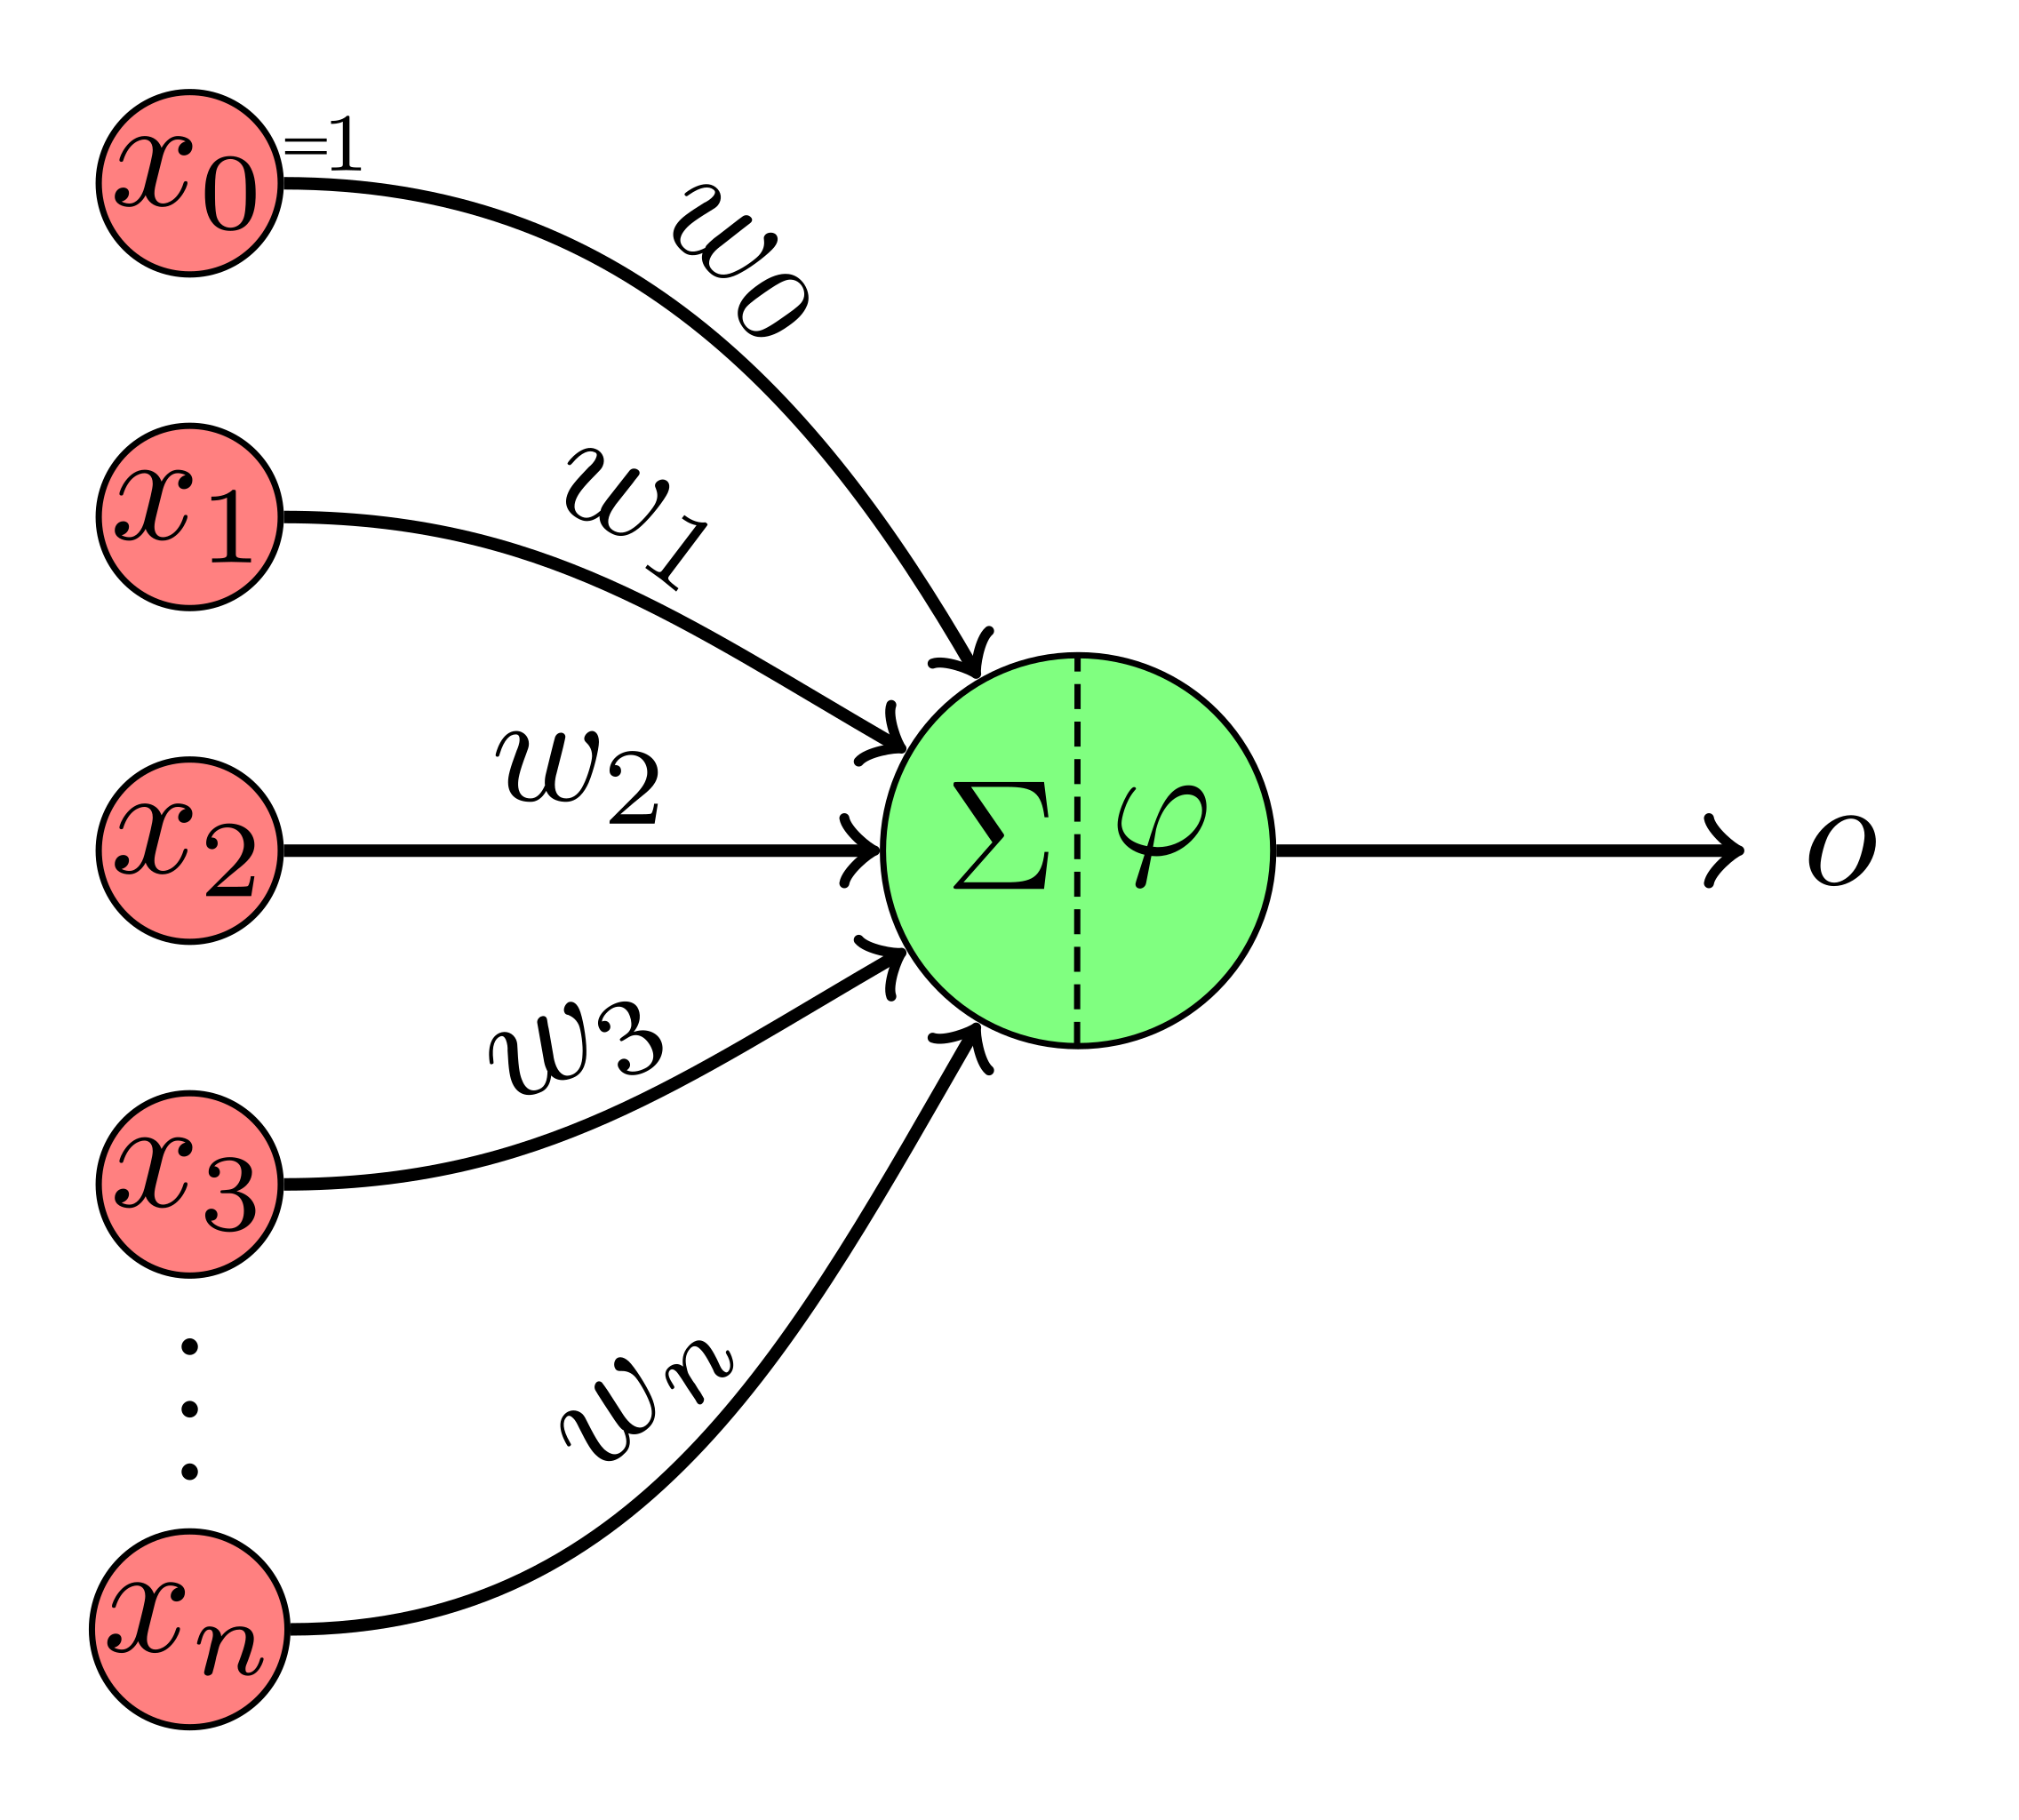
\includegraphics[width=0.5\textwidth]{figures/perceptron.png}
%  \end{center}
%  \caption{Model of a perceptron.}
%  \label{fig:perceptron}
%\end{figure}

%\begin{center}
%Bias is omitted in this figure.
%\end{center}

%To solve more complex problems than binary classification problems in a linearly nonseparable vector space one has to alter the activation function and in many cases use a deeper and wider ensemble of perceptrons. Depending on the activation function used, the perceptron can output a different range of values. Traditionally a very popular activation function was the non-linear \textit{sigmoid activation function}. Lately, due to the problems with vanishing gradients (which we will cover shortly) the piecewise linear function \textit{Rectified Linear Unit} (ReLU) is the standard activation function today.

%Perceptrons can be stacked after and next to one another (in the latter case known as a layer), called a multi-layer perceptron (MLP). The first layer, where the input signal is the input data itself, represented in floating point numbers, is called the input layer. The last layer, where the output signal corresponds to the decision or classification, is called the output layer. Any layer between the input layer and the output layer is called a hidden layer. Together these layers form what is known as an Artificial Neural Network. Any ANN with at least two hidden layers is called a Deep Neural Network (DNN).



\subsection{Training a Deep Neural Network}

Neural networks can learn to approximate functions through learning. Learning occurs by updating the weights and biases of the perceptrons gradually to approximate the desired output value of the last layer in the neural network. This difference between the desired output value and the output of the network, also known as the cost, is estimated by using a cost function. Cross-entropy is a popular cost function. In \autoref{eqn:crossentropy}, \(y\) is the true label, and \(\hat{y}\) is the predicted value of the current model.

\begin{equation}
    cost(y, \hat{y}) = - \sum\limits_{i=1}^{n} y_i log(\hat{y_i})
    \label{eqn:crossentropy}
\end{equation}

By updating the weights according to a paradigm, the cost can be minimized. A gradient-based approach to minimizing the cost is called backpropagation~\cite{Rumelhart1986}. Backpropagation is defined as taking the following steps:

\begin{enumerate}
\item Forward the input through the neural network to generate a prediction $\hat{y}$.
\item Measure the cross-entropy loss e.g. according to \autoref{eqn:crossentropy}
\item Propagate back the error’s gradient from the last(output) to the first(input) layer of the network.
\item Change the weights and biases based on the gradient.
\end{enumerate}

The error or loss can be calculated according to \autoref{eqn:crossentropy} as such:

\begin{equation}
    J(w_j) = cross\_entropy(y_j,\hat{y_j}) = - \sum_{j} y_j log(\hat{y_j})
    \label{eqn:jacobian}
\end{equation}


where $w_j$ is the weights of the DNN at layer $j$ and $\hat{y}$ can be seen as a non-linear function of the weights. The updated weight values can be seen in \autoref{eqn:weights}.

\begin{equation}
    w_{i,j}^{(next)} = w_{i,j} - \eta \frac{\partial J(w_j)}{\partial w_i}
    \label{eqn:weights}
\end{equation}

To update the weight $w_{i,j}$ using gradient descent, a \textit{learning rate} $\eta > 0$ must be chosen. Each value of the updated weights in the next layer depends on the partial derivative of the previous layer. That is why each activation function has to be differentiable (Nevertheless, the ReLU activation function is non-differentiable at 0), and why the error has to be \textit{propagated backwards}.

\textbf{Should this be explained in more detail? Cases where the $w_i$ is an output neuron vs hidden. }

\subsection{Challenges in training}

In real world applications, there are many challenges when training a deep neural network.

\subsubsection{Overfitting/underfitting}

With a large number of parameters, the network can be said to have a high degree of freedom. It becomes so complex that it will encounter the overfitting problem~\cite{doi:10.1021/ci0342472}. Overfitting means that the network will tend towards having lower accuracy of the test dataset, despite an increasing accuracy on the training dataset. This phenomenon can be anecdotally compared to memorizing the training dataset by heart, and thus losing the generalization property when tested on data outside the training dataset.

\begin{figure}[H]
  \begin{center}
    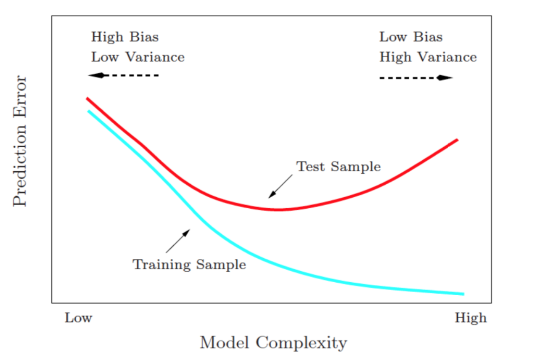
\includegraphics[width=0.8\textwidth]{figures/overfitting.png}
  \end{center}
  \caption{Model complexity and overfitting~\cite{Wang_2019}. }
  \label{fig:overfitting}
\end{figure}

Several approaches can be taken to minimize or resolve the problem of overfitting.
\begin{enumerate}
\item Regularization~\cite{10.1038/317314a0}: By imposing a cost (or penalty) on the optimization function, the optimal solution can be made unique.
\item Early stopping~\cite{Prechelt2012}: By halting the training when the error of the test dataset reaches its minimum, overfitting can be avoided. Early stopping can be thought of as regularization in the temporal domain.
\item Dropout~\cite{JMLR:v15:srivastava14a}: By randomly ignoring some neurons during training to reduce the model complexity, an increase in model sparsity is gained.
\item Data augmentation~\cite{10.2307/2289457}: Additional data is created, typically in preprocessing, by altering the original data in a number of ways which are added in addition to the original data. For visual data, some examples are: changing angles, illumination, saturation, exposure, etc. This creates additional variance which prevents simply memorizing shallow features in the dataset.
\end{enumerate}

\subsubsection{Exploding/vanishing gradients}
When the backpropagation algorithm backflows the error gradient from the output layer back towards the input layer, the gradient will diminish by the layer if the initial gradient is smaller than 1.0, and increase substantially when initially greater than 1.0. As a result, some parameters will either remain unchanged by the diminished gradient or changed by a large value by the time the update process reaches very deep in large networks.

Some techniques for overcoming the exploding/vanishing gradient problem are~\cite{doi:10.1142/S0218488598000094}:

\begin{enumerate}
\item Non-saturating activation functions: Using e.g. ReLU~\cite{maas2013rectifier} instead of the commonly used sigmoid activation function can help during training. The gradient is minimal when the sigmoid function is close to its output limits $(-1/1)$ meaning it will saturate. Using ReLU = $max(0,z)$ won't have this problem. However, ReLU has its own problem in that some perceptrons may stop outputting values except for 0. This is known as the dying ReLU problem. The solution is to use leaky ReLU = $max(az,z)$ where $a$ is the slope when $z < 0$.

\begin{figure}[H]
  \begin{center}
    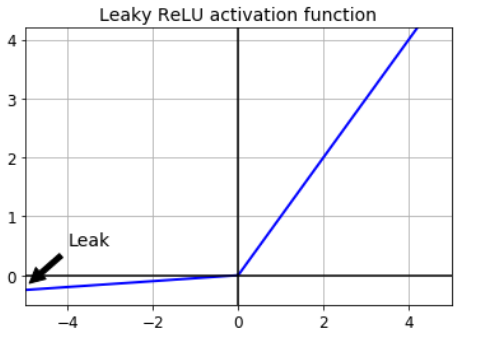
\includegraphics[width=0.7\textwidth]{figures/leaky_relu.png}
  \end{center}
  \caption{Leaky ReLU~\cite{Wang_2019}.}
  \label{fig:leaky_relu}
\end{figure}

\begin{center}
The leaky ReLU activation function prevents the \textit{dying ReLU problem}.
\end{center}

\item Gradient clipping~\cite{quintana1974clipping}: Clipping the gradient by defining a max value it can attain during backpropagation means it will never exceed a certain threshold. This solves the exploding gradient problem.

\item Batch Normalization~\cite{ioffe2015batch}: A technique used to address the problem that the distribution of each layer’s inputs changes during training, as the parameters of the previous layers change, by zero centering the input, scaling and then shifting the result. Due to the impracticality of using the global information for normalization, each normalization occurs at each mini-batch $B$ of size $m$. The mean $\mu_{B}$ and variance $\sigma_B^2$ can be calculated as follows:

\begin{equation}
    \mu_B = \frac{1}{m_B} \sum_{i=1}^{m_B} x^{(i)}
    \label{eqn:bnmean}
\end{equation}

And thus follows the calculation of the \textit{variance} $\sigma_B^2$ of $B$:

\begin{equation}
    \sigma_B^2 = \frac{1}{m_B} (x^{(i)} - \mu_B)^2
    \label{eqn:bnvariance}
\end{equation}

For a layer of the network with d-dimensional input, $ x = (x^{(1)}, ..., x^{(d)}) $, each dimension of its input is then normalized (re-centered and re-scaled) separately:

\begin{equation}
    \hat{x}_{i}^{(k)} = \frac{x_{i}^{(k)} - \mu_{B}^{(k)}}{\sqrt{\sigma_{B}^{(k)^2} + \epsilon}}
    \label{eqn:bnorm}
\end{equation}

where $\epsilon$ is an arbitary small constant added for numerical stability.

\end{enumerate}
\subsubsection{Improving gradient descent}

Training speed can be improved by using techniques to update the learning rate during training, making the model converge faster towards the desired weight distribution.
\begin{enumerate}
\item Momentum~\cite{Rumelhart1986}: In order to improve an otherwise static learning rate, momentum was introduced by Rumelhart, Hinton and Williams. The idea is to remember the update $\Delta w$ at each iteration, and determine the next update as a linear combination of the gradient and the previous update:

\begin{equation}
    w = w - \eta \nabla Q_i(w)- \alpha \Delta w
    \label{eqn:momentum}
\end{equation}

where the parameter $w$ which minimizes $Q(w)$ is estimated, $\eta$ is the learning rate, and $\alpha$ is an exponential decay factor between 0 and 1.

\item Weight decay~\cite{DBLP:journals/corr/abs-1711-05101}: When using stochastic gradient descent (and rescaling with the learning rate), weight decay
is a form of regularization which adds a penalty term to the loss in order to encourage the model to select smaller or sparser weights,
depending on whether one uses $L_1$ or $L_2$ weight decay.

\end{enumerate}


\subsection{Convolutional Neural Network}

Traditional DNNs had, at the time of creation, very impressive results on many datasets and tasks. However, working with 2-D images, certain problems arose related to the architecture. Traditional MLPs encountered difficulty with learning spatial and translation features, such as lighting or distortion variance. The difficulty in learning spatial features is directly related to how DNNs treat each pixel individually as an input vector and thus losing spatial information on how pixels relate to each other.

\textbf{Convolutional layer}. A 2-D image consists of 3 dimensions: The width, height and channels (Typically 3: Red, green and blue). The convolutional layer, when applying its operation to the input, slides across the image (also referred to as convolves) from the top left corner to the bottom right corner as depicted in \autoref{fig:kernelmovement}, performing a matrix multiplication operation between the kernel(a matrix of weights) and the portion of the image it is currently located at. Each kernel operation produces a number(after a bias value is added) which is inserted into a resulting matrix, named a \textit{filter}.

\begin{figure}[H]
  \begin{center}
    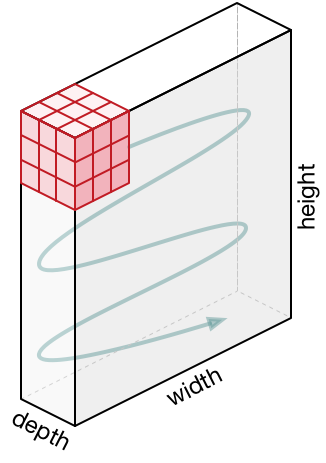
\includegraphics[width=0.5\textwidth]{figures/kernel_movement.png}
  \end{center}
  \caption{Movement of the kernel within the input image or filter matrix~\cite{Kang2020DeepCN}.}
  \label{fig:kernelmovement}
\end{figure}


Options for determining the resulting output size of the convolutional layer are called \textbf{stride} and \textbf{zero-padding}. Stride determines how many pixels the kernel shifts as it traverses. Increasing the stride will decrease the number of operations performed, and thus the output size.

Since the kernel will pass the border of the image input fewer times than the pixels located closer to the center of the image, zero-padding can be used to improve the performance of the convolutional layer. Zero-padding adds zeros to the edges of the image, making it possible to traverse the original corners and borders of the image multiple times. The logical consequence of artificially increasing the width and height of the image is that more convolves occur, and thus the output size of the layer is increased.

\begin{figure}[H]
  \begin{center}
    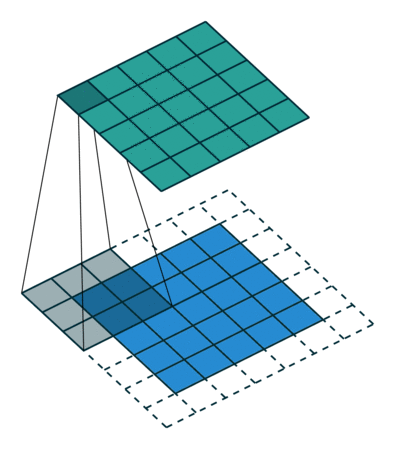
\includegraphics[width=0.5\textwidth]{figures/padding.png}
  \end{center}
  \caption{Zero-padding~\cite{Kang2020DeepCN}.}
  \label{fig:padding}
\end{figure}

\begin{center}
Zero-padding the image input (in blue and on bottom) by 1 makes the convolutional layer produce the same output dimensions(green and on top) as the input. When the same dimensionality is produced, it is known as \textbf{same-padding}.
\end{center}

\textbf{Pooling layer.} Similar to how convolutional layers work, pooling layers are responsible for reducing the spatial size of the convolved features. This is to decrease the computational power required to process the data through dimensionality reduction. Another feature of the pooling layers is that, as we reduce the dimensionality of the layers further down the architecture, we force the layers to learn on higher and higher levels of abstraction of the features, since detail is lost with the compression of information. There are two important types of pooling layers: \textbf{Max pooling} and \textbf{average pooling}. As the names suggest, the operation applied to inputs of the layers is the maximum of the values or the average of the values respectively.

\textbf{Dense layer}. Typically in these architectures, the final layers are traditional dense layers. These layers are used to output the probability of a certain class to be detected within the image.

\textbf{Residual block}. As networks became deeper to improve results, the problems with vanishing and exploding gradients became more commonplace again. Residual neural network (ResNet), was proposed by Kaiming He et al~\cite{he2016deep}. It’s main contribution to the CNN architecture was the residual block, which introduced a short cut layer in order to improve learning as seen in \autoref{fig:residual}.

\begin{figure}[H]
  \begin{center}
    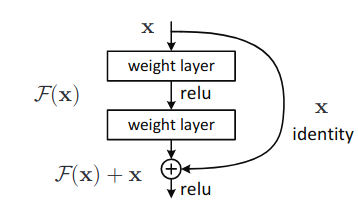
\includegraphics[width=0.7\textwidth]{figures/residual_block.png}
  \end{center}
  \caption{Residual block~\cite{he2016deep}.}
  \label{fig:residual}
\end{figure}

\subsection{Fully Convolutional Network}

Achieving state-of-the-art results on PASCAL VOC~\cite{DBLP:journals/corr/LongSD14}, among other datasets, at the time of creation, Fully Convolutional Networks (FCN) output a per-pixel prediction of the segmentation by first convoluting the features and then de-convoluting back to the original size of the input layer as can be seen in \autoref{fig:fcn}.

\begin{figure}[H]
  \begin{center}
    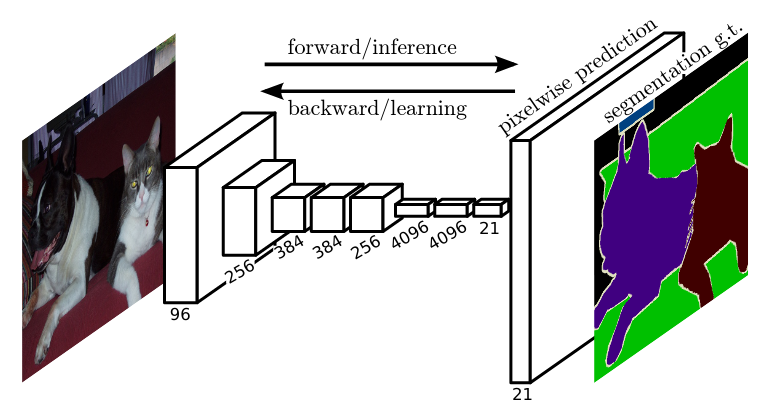
\includegraphics[width=1.0\textwidth]{figures/fcn.png}
  \end{center}
  \caption{Fully Convolutional Network architecture as depicted in the original paper~\cite{DBLP:journals/corr/LongSD14}.}
  \label{fig:fcn}
\end{figure}

This is done by removing the final classifier layer and converting all fully connected layers to convolutions. They then append a $ 1 x 1$ convolution with channel dimensions $N$ where $N$ is the number of classes for the specific dataset, followed by a \textit{deconvolution} layer to bilinearly upsample the coarse output to pixel-dense outputs.

The deconvolution layer simply reverses the process of the convolutional layer, explained previously in this chapter.

\subsection{Feature Pyramid Network}

Recognizing objects at vastly different scales is one of the fundamental challenges in computer vision. One approach which has proven to be successful in both performance on competitive datasets (e.g. the MS COCO detection benchmark without bells and whistles\footnote{Bells and whistles are classes that are excluded in their performance benchmark.} in this case) and in the sense that it adds little overhead, is the Feature Pyramid Network (FPN). The idea is intuitive: To offset the problem of objects being of vastly different scales in images, the features maps generated from the images are scaled to different resolutions as seen in \autoref{fig:fpn}, and predictions are made on each of these scaled feature maps.

Previous approaches similar to the FPN also leverage the pyramid scheme to predict objects at different resolutions. However, as in the case of Featurized image pyramid a) in \autoref{fig:fpn}, inference time could increase by up to four times making the approach impractical for real world applications.

Convolutional neural networks typically narrow it’s hidden layers in common architectures, either to make a prediction based on high-level features as in the case of the common heads used in the R-CNN family of networks, or in the case of FCNs, where the layers typically decrease in size only to increase towards the output layers in order to produce a proposal of equal dimensions as the input layer. FPNs exploit the architecture of the CNNs by using the existing hidden layers at different resolutions to predict bounding boxes and classes directly from the hidden layers, reducing the overhead of the FPN backbone, and thus becoming a feasible option for real world applications.

\begin{figure}[H]
  \begin{center}
    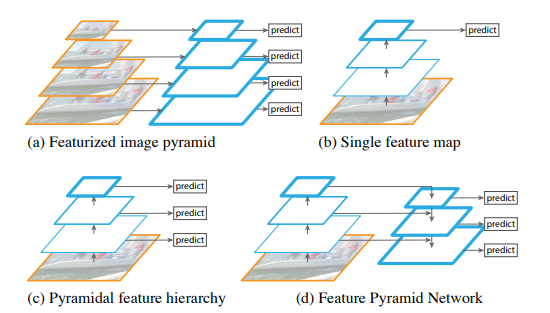
\includegraphics[width=1.0\textwidth]{figures/fpn.png}
  \end{center}
  \caption{Evolution of the Feature Pyramid Network~\cite{DBLP:journals/corr/LinDGHHB16}.}
  \label{fig:fpn}
\end{figure}

\subsection{Mask R-CNN}
\label{subs:maskrcnn}

Mask R-CNN is a deep learning neural network architecture designed for object instance detection and segmentation. Given an input image, the network produces bounding boxes, segmentation masks, and an estimated class for each object detected in the image. Mask R-CNN is an extension in a longer line of extensions of neural network architectures.

\textbf{R-CNN}. The reason the original CNN is not ideal to use for object detection in images is that the output may be variable since you might have a variable amount of objects being detected in the image, making the output size vary from one image to the next. Region Based Convolutional Neural Network (R-CNN), proposed by Ross Girshick et al~\cite{Girshick_2014_CVPR}, uses a method where selective search is used to extract 2000 regions from the image called region proposals. Each proposal is warped into a square and fed into a CNN that produces a 4096-dimensional feature vector as output. In this case, the CNN acts as a feature extractor and the output dense layer consists of the features extracted from the image. These features are fed into a Support Vector Machine to classify the presence of an object within the region proposal. The algorithm also predicts four values which are offset values to increase the precision of the bounding box.

\textbf{Fast R-CNN}. The next evolution of the R-CNN, called “Fast R-CNN”~\cite{Girshick_2015_ICCV}, hints at the problems that R-CNN had and that its extension is trying to solve. R-CNN took a very long time to produce its output, and the selective search algorithm used to propose the regions is fixed, neglecting the possibility to learn in this stage of the architecture. Fast R-CNN introduces a RoI (Region of Interest) pooling layer, making it possible to skip generating 2000 region proposals and instead only have the convolution operation done once per image.

\textbf{Faster R-CNN}. Fast, but not fast enough, the Fast R-CNN still took a significant time generating the region proposal, albeit much faster than its predecessor. Shaoqing Ren et al~\cite{7485869} came up with a replacement for the selective search algorithm with the added bonus that it lets the network learn in the region proposal step. This part of the network is called the Region Proposal Network (RPN).

\textbf{Mask R-CNN}. Mask R-CNN contributes to this architecture by adding a parallel prediction of masks alongside its original output which is a class label and a bounding-box offset. This parallel proposal is what made Mask R-CNN unique compared to other extensions of Faster R-CNN at the time, where other methods often depended on the mask predictions for the class prediction. Mask R-CNN also introduces the concept of RoIAlign, to address misalignment issues between the RoI and the extracted features which impacts the pixel-accurate masks it produces due to quantization which is avoided with RoIAlign. More thorough details can be found in the original Mask R-CNN paper, He et al~\cite{DBLP:journals/corr/HeGDG17}. All deviations from the standard configuration will be noted in \autoref{ch:method}.

\textbf{Weaknesses of Mask R-CNN}.
M. Kisantal et al~\cite{DBLP:journals/corr/abs-1902-07296} describe a problem for Mask R-CNN in the fact that it struggles to perform well on small objects.
There are a number of factors that contribute to this deficit.

Firstly, in the MS COCO dataset, the number of images with small objects are significantly fewer than the number of images with medium or large objects ($51.82\%$ vs $70.07\%$ and $82.28\%$ respectively).

The total annotated pixels per object size also differs significantly ($1.23\%$ vs $10.18\%$ and $88.59\%$ respectively).

Lastly, each predicted anchor from the RPN receives a positive label if it has the highest IoU with a ground truth bounding box or if it has an IoU higher than 0.7 for any ground truth box. As the authors describe, this procedure favors large objects because "A large object spanning multiple spanning-window locations often has a high IoU with many anchor boxes, while a small object may only be matched with a single anchor box with a low IoU".

\subsection{Microsoft COCO: Common Objects in Context}

The Microsoft COCO: Common Objects in Context or MS COCO is a dataset for object recognition, classification and semantic segmentation.
It contains 328k images, 2.5 million labeled instances and 91 object types grouped in 11 super-categories.
As the name suggests MS COCO is described as "a collection of objects found in everyday life in their natural environments", as seen in \autoref{fig:mscoco}.
The resolution of the images found in the dataset are $640$x$480$ pixels.

\begin{figure}[H]
  \begin{center}
    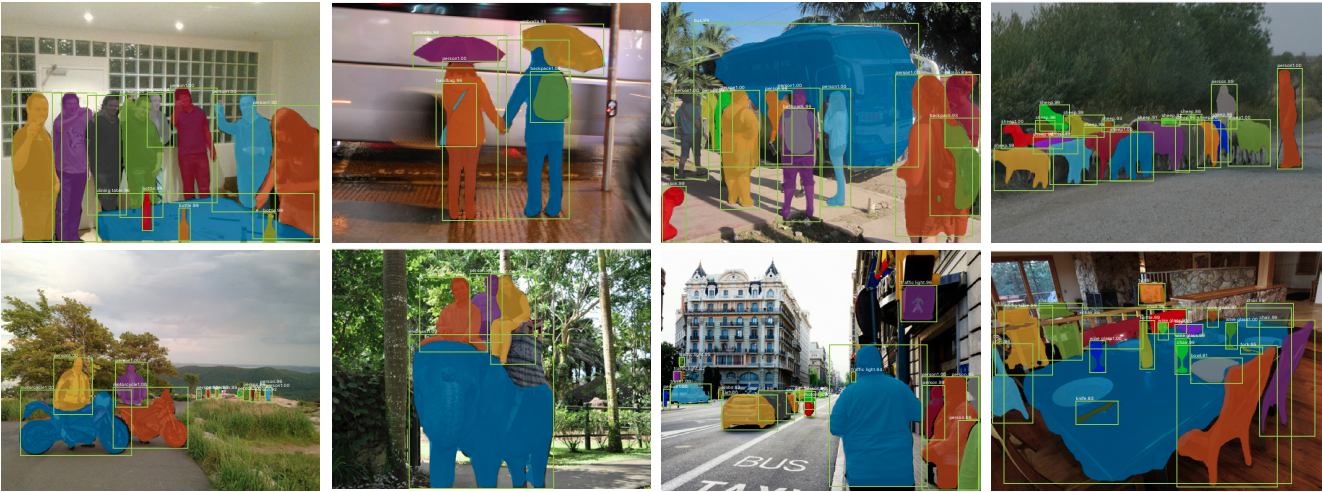
\includegraphics[width=1.0\textwidth]{figures/mscoco.png}
  \end{center}
  \caption{Mask R-CNN results on the MS COCO dataset~\cite{DBLP:journals/corr/HeGDG17}. Masks are shown in color. Bounding boxes, category and confidence are also shown.   }
  \label{fig:mscoco}
\end{figure}


\section{Related work: Segmentation Algorithms}
\label{sec:relwork}

In the survey "A comprehensive survey of mostly textual document segmentation algorithms since 2008"~\cite{ESKENAZI20171} a topology for organizing segmentation algorithms is introduced based on the details of the algorithmic approach.

According to this survey, three groups of approaches can be identified:

\begin{enumerate}
\item Top-down
\item Bottom-up
\item Hybrid algorithms
\end{enumerate}

We will first review the classical algorithms, which are typically constrained by either the layout of the document (Such as the Manhattan layout\footnote{The Manhattan layout assumes that all text lines can have one of two orientaitions (horizontal or vertical) after affine corrections.}~\cite{395720}) or parameters of said document (Such as font size or line spacing), and finally review the previous works in the domain of deep learning, which belong to the hybrid algorithms.

Each algorithm noted in the following chapter is classified depending on from which perspective it starts it's processing. Top-down algorithms start from the whole page, partitioning into smaller and smaller parts. On the contrary, bottom-up algorithms try to agglomerate elements into bigger and bigger elements up towards the whole page. See \autoref{fig:classicalgs} for a complete picture.

\subsection{Classical Approaches}

\textbf{Layout constrained algorithms}. The first algorithms to appear in semantic segmentation tasks usually made strong assumptions about the layout of the documents. The algorithms can be further categorized into three groups based on how they assume the layout as can be seen in \autoref{fig:classicalgs}.

The earliest attempts at semantic segmentation made clear assumptions about the document layout, either with grammar (a set of rules), or by assuming the Manhattan layout and using projection profiles.

Second came the algorithms that rely on Run-Length Smoothing Algorithm (RLSA), mathematical morphology or other filters. The characteristics of these filters reflect the assumptions made on the layout geometry.

Lastly, algorithms focused on detecting straight lines or square borders appeared e.g. using the Hough transform. This includes detecting white space alignment in which case the lines may appear “invisible”.

\textbf{Parameter constrained algorithms}. Moving away from the rigid assumptions, the second group of algorithms try to adapt to local variations in the document in order to be able to segment a broader range of layouts without changing the algorithm itself. The drawback of these techniques is the increased complexity and number of parameters associated with the algorithms. These parameters can be difficult to tune and may require larger datasets to train on. In this group we find the clustering algorithms, the algorithms based on function analysis, and the classification algorithms.

Finally, in an attempt to overcome the limitations of the already mentioned algorithms, several techniques are combined in hybrid algorithms. Thus they cannot be categorized as either bottom-up or top-down algorithms since they may be both.

\begin{figure}[H]
  \begin{center}
    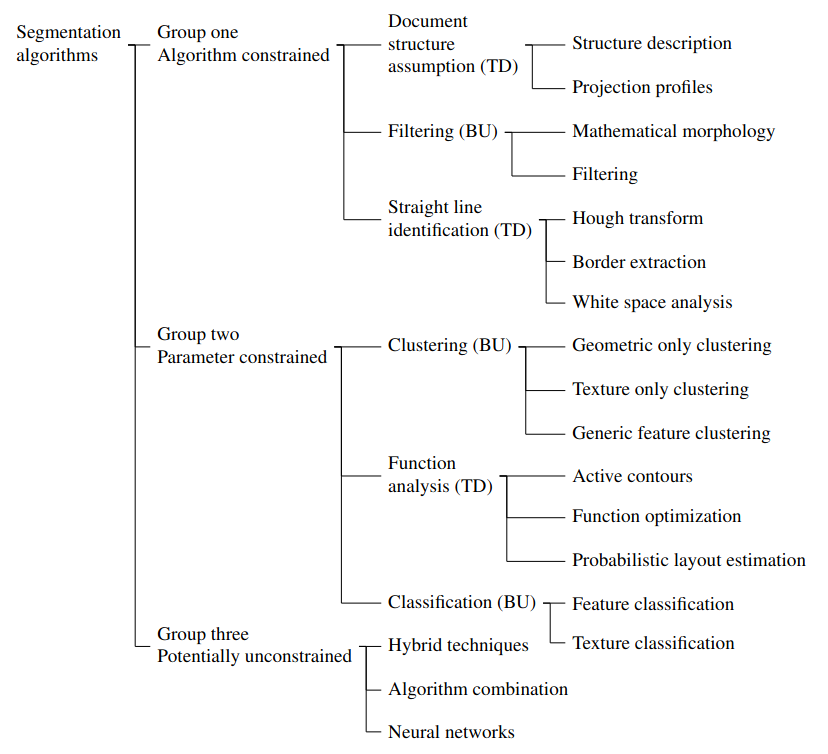
\includegraphics[width=1.0\textwidth]{figures/classicalalgs.png}
  \end{center}
  \caption{Hierarchical typology of document segmentation algorithms~\cite{ESKENAZI20171}.   }
  \label{fig:classicalgs}
\end{figure}

\begin{center}
Top-down (TD) and bottom-up (BU) algorithms are also denoted.
\end{center}

\subsection{Deep Learning Approaches}
\label{subs:dlapproaches}

In an attempt to trade prior handcrafted features for learning capabilities, machine learning techniques, especially deep neural networks have outperformed classical algorithms in recent papers. These approaches can be categorized by the input they receive.

\textbf{Image modality only}. Convolutional neural networks were originally created to classify objects in images such as hand written numbers by LeCun et al~\cite{lecun1989}. Since then, CNNs are used in a wide variety of image classification domains~\cite{deng2009}. Since CNNs can use images as input to the network, they naturally lend themselves to be applied in this domain as well. Attempts have been made~\cite{DBLP:journals/corr/0011S17}, as well as several variants~\cite{he2017, xu2017, wickpuppe2018, oliveira2018} of the Fully Convolutional Network (FCN) introduced by Long et al~\cite{DBLP:journals/corr/LongSD14}. The major drawback of these techniques is that they do not exploit the often available localized, two-dimensional, textual input obtained through OCR scanning.

\textbf{Image and text modalities}. The representation of text as input to deep neural networks has increased in complexity since it was first tried in Meier et al~\cite{8270006} using a FCN based approach. In this attempt, the textual information was represented as a binary feature (a pixel has text or not), where lexical and semantic dimensions are not taken into account.

Katti et al~\cite{katti2018} introduced the concept of \textit{chargrid}, a two dimensional representation of text where characters are localized on the image and encoded as a one-hot vector. This study shows that model variants exploiting both modalities achieve better results, at the cost of high-computing. While Dang and Nguyen Thanh~\cite{DBLP:journals/corr/abs-2106-00952} build on this approach and show an impressive mIoU of 87\% for template-like administrative documents, Denk and Reisswig~\cite{DBLP:journals/corr/abs-1909-04948} (who also build upon Katti et al~\cite{katti2018}), consider not only characters, but words and their corresponding embeddings. Using BERTgrid for the automatic extraction of key-value information from invoice images (amount, number, date, etc), they obtain the best results with document representation based on one-hot character embedding and word-level BERT embeddings with no image information.

Moving from character, to word, to sentence representations, Yang et al~\cite{DBLP:journals/corr/YangYAKKG17} represent text via text embedding maps, where the two-dimensional text representation is mapped to the pixel information. Textual features correspond to sentence embeddings in this case, with the use of word vectors obtained with Word2Vec~\cite{mikolov2013} and averaged in the final embedding.

Finally, Barman et al~\cite{jdmdh:7097} combine word embeddings with a deep neural network approach specifically within the domain of newspaper segmentation. The critical difference to this paper is that Barman et al~\cite{jdmdh:7097} uses word embeddings, where we will vary difference sentence embedding encoders. The primary architecture used in Barman et al~\cite{jdmdh:7097} is dhSegment, where we will vary different settings within the newer architecture Mask R-CNN, developed specifically for instance segmentation. Similarly to Barman et al~\cite{jdmdh:7097}, we will modify the architecture to fit the text embeddings behind the image pixels by extending the number of channels in the image and inserting the text embeddings at the coordinates of the text bounding box produced by the OCR.

\section{Related work: Word representation language models}
\label{sec:langrep}

In the survey "A Comprehensive Survey on Word Representation Models: From Classical to State-of-the-Art Word Representation Language Models" by Naseem et al~\cite{10.1145/3434237} a variety of different word representation langauge models are detailed.

\subsection{From classical methods to state-of-the-art}

What follows is a historical review of the methods to represent textual information for many downstream Natural Language Processing (NLP) tasks, such as sentence similarity, which relates to the goal of the proposed architecture in this thesis. 

\subsubsection{Categorical word representation}

The simplest way to represent text as a feature vector is to use categorical word representation. Two models that use categorical word representation are one hot encoding and bag-of-words (BoW). 

In \textbf{one hot encoding} words are represented as either a $1$ or a $0$. The vector length or \textit{dimension} of the feature vector is equivalent to the number of terms in the vocabulary. 

 \textbf{Bag-of-words} is an extension of the one hot encoding. Instead of representing terms as prevalent or not ($1$ or $0$), BoW represents occurences of the terms, the number representing the prevalence of a term is equal to the number of times it occurs in the text.

\subsubsection{Weighted Word representation}

Instead of representing only the prevalence or the number of times a term appears in a text, weighted models represent term based on its frequency in relation to the total number of terms in the document. 

\textbf{Term Frequency} (TF) calculates the number of times a term appears in a text divided by the total number of terms in the text.

\textbf{Term Frequency-Inverse Document Frequency} (TF-IDF) reduces the impact of common words, known as \textit{stop words}. The Inverse Document Frequency divides the number of documents by the number of documents in which the term appears, which is then logarithmically scaled. 

\begin{equation}
	tfidf(t,d,D) = tf(t,d) * idf(t,D)
  	\label{eqn:tf-idf}
\end{equation}


\begin{equation}
	tf(t,d) = \frac{f_{t,d}}{\sum_{t' \in d} f_{t', d}} 
  	\label{eqn:tf}
\end{equation}

Where $f_{t,d}$ is the number of times that the term $t$ occurs in the document $d$, and $\sum_{t' \in d} f_{t', d}$ is the number of terms $t'$ in the document $d$.

\begin{equation}
	idf(t,d,D) = log \frac{N}{|d \in D : t \in d|}
  	\label{eqn:idf}
\end{equation}

Where $N$ is the total number of documents in the corpus and $|d \in D : t \in d|$ is the number of documents where the term $t$ appears. Usually a constant term of $1$ is added to the denominator to avoid division by zero if the term is not in the corpus.

\subsubsection{Word embeddings}

The aforementioned methods have drawbacks. Vector representation where each term is assigned its own index results in large dimensional arrays for large text corpora. Given that many terms may not appear in every document, the resulting representation can be said to be sparse. Furthermore, information is lost in this type of representation in regards to order of terms, as well as any information of the grammar used in the sentences.

Since these models fail to capture syntactic and semantic meaning of words as well as suffer from the curse of high dimensionality, new methods like word embeddings have replaced categorical text representation methods for tasks in the domain of NLP.

These models have been replaced by \textit{feature learning} or \textit{representation learning} using supervised or unsupervised neural network based methods.

Word embedding is a feature learning method where a term from the vocabulary is mapped to a $N$ dimensional vector. Word2Vec, GloVe, and FastText are some of the models that use word embeddings to represent features.

\textbf{Word2Vec}~\cite{mikolov2013} is a shallow neural network model for learning feature representations of words. It creates word representations using two hidden layers captured by either Continuous Bag of words (CBOW) or Skip-gram. Training is done using a local context window of predefined length. 

\textbf{Global Vectors}\cite{pennington2014glove} (GloVe) is an expansion of the Word2Vec architecture where a local context window is extended by an additional global matrix factorization, becoming a global log-bilinear regression model.

Both Word2Vec and GloVe are better at learning the semantic representation of words compared to categorical word representation and weighted word representation since they attempt to capture the context of nearby words in the learning procedure. Neither can however learn representations of words out-of-vocabulary. 

\textbf{FastText}~\cite{DBLP:journals/corr/BojanowskiGJM16} is an attempt to improve previous architectures by also learning the word representations with regards to the morphology of words. It is based on the Skip-gram model, where each word is represented as a bag of character $n$-grams. It allows for computation of word reperesentations for words that did not appear in the training data. 

\subsection{BERT}

The Bidirectional Encoder Representations from Transformers~\cite{devlin2018bert} (BERT) is a multi-layer bidirectional Transformer~\cite{46201} encoder that is an extension of the OpenAI Generative Pre-training Transformer model~\cite{radford2018improving}  (GPT) Transformer architecture. Unlike GPT however, BERT uses bidirectional self-attention, while GPT uses constrained self-attention where every token can only attend to context to its left.

Pre-trained BERT models can be fine-tuned with just one additional output layer to create state-of-the-art models for a wide range of tasks, such as question answering and language inference, without substantial architecture modifications.

\subsection{Sentence-BERT}

Sentence-BERT~\cite{reimers-2019-sentence-bert, reimers-2020-multilingual-sentence-bert} (SBERT) is a modification of the pretrained BERT model that uses siamese and triplet network structures to derive semantically meaningful sentence embeddings that can be compared using cosine-similarity for tasks of Semantic Textual Similarity (STS). 

Sentence-BERT is the chosen architecture for generating sentence embeddings in this thesis. As a final note for this section, on the topic of what a \textit{sentence} is in the context of BERT:


\begin{displayquote}
Throughout this work, a “sentence” can be an arbitrary span of contiguous text, rather than an actual linguistic sentence.~\cite{devlin2018bert}
\end{displayquote}

\textbf{TODO abbreviations for this section}

\section{Summary}

In this chapter we have reviewed the necessary preliminaries for understanding the work done in this thesis. We have reviewed the history of semantic segmentation, the history of word representation language models, the data we are about to present methods and results for, as well as the preliminaries for understanding the challenges of working with neural networks in this context.

\clearpage


\chapter{Method}
\label{ch:method}

\section{System documentation}
\label{sec:sysdoc}

This chapter lists the versions and specifications for reproducibility purposes.

\subsection{Hardware specifications}

\textbf{TODO computer specs, maybe even model sizes in memory and running time for training?}


\begin{table}[!ht]
  \begin{center}
    \caption{Hardware specifications}
        \begin{tabular}{l*{6}{c}r}
        \label{tab:hardwarestats}
        \textbf{Component} & \textbf{Specification} & \\
        \hline
        CPU & Intel® Core™ i7-7820X CPU @ 3.60GHz × 16 & \\
        GPU & NVIDIA GeForce RTX 3090 & \\
        RAM & 125 GB \\
        \end{tabular}
  \end{center}
\end{table}


\subsection{Software specifications}

\subsubsection{MMDetection}
The MMDetection~\cite{DBLP:journals/corr/abs-1906-07155} framework was used to conduct the experiments in \autoref{sec:experiments}.
MMDetection is an object detection toolbox in which includes training and inferences codes, in addition to weights for over 200 network models.

MMDetection allows for inheritance of configuration files, making it possible to conduct various experiments while varying small parts of the code.
In addition to modular config loading, the parameters can also be inserted at runtime to reduce the amount of static files needed to vary hyperparameters.

\subsubsection{Label studio}
Label studio~\cite{Label_Studio} was used to produce the labels for the datasets created in this thesis. In the interest of time and precision of the labels, the labels were first created using rectangles, exported, converted to polygons, and then imported again to be reviewed and edited where necessary. 

\subsubsection{Software versions}

The following is a complete list of versions of software used in this thesis.

\begin{table}[!ht]
  \begin{center}
    \caption{Software versions}
        \begin{tabular}{l*{6}{c}r}
        \label{tab:softwareversions}
        \textbf{Software} & \textbf{Version} \\
        \hline
        Ubuntu & 20.04.3 LTS & \\
        Nvidia driver     & 470.86 & \\
        Python           & 3.8.11 & \\
        CUDA     & 11.4 & \\
        cudatoolkit     & 11.3.1 & \\
        tensorflow (-gpu)     & 2.5.0 & \\
        torch (vision)     & 0.9.0+cu111 & \\
        MMDetection (mmdet)     & 2.18.0 & \\
        Label Studio     & 1.2 & \\
        \end{tabular}
  \end{center}
\end{table}

\section{Data}

A description of the labeling strategy will be introduced, as well as the caveats that arise from working with newspaper data.
Each class will be described and any special delimitations will be detailed.

Definitions will be based on what a user might like to query as content on an article-level search of a newspaper.
Because of this rather subjective definition, a systematic description of how elements of units are labeled will be produced in this chapter.

\subsection{Labeling strategy}
\label{subsec:labelingstrat}

In this thesis we are concerned with grouping elements together that relate by their contents.
For example, a news article might have an image depicting the contents, a title, a body of text possibly spanning multiple text blocks, and a byline.
These elements together form one \textit{instance} of a class.

Some elements of the newspaper do not by themselves convey any news. One example are elements used for navigating the newspaper itself.
Such elements include titles, section titles and subsection titles. Another example could be instructions for participating in debate, or footers that present the newspaper publishing team.
These elements are considered \textit{static} and receive no label in this thesis.

The label bounding box will be the smallest spanning bounding box, including white spaces between the elements, should they make up a rectangular shape.
In the case that elements are organized such that they do not make up a rectangular shape, a smallest rectangular shape will be made excluding the protruding elements,
which are then included by extending the border of the original rectangular shape in an asymmetric manner as can be seen in \autoref{fig:asymextention}.

\begin{figure}[H]
\label{fig:asymextention}
\begin{tikzpicture}
\draw[step=1cm,white,very thin] (-2.9,-2.9) grid (6.9,6.9);
\draw[red] (-2,-2) -- (2,-2) -- (2,4) -- (6,4) -- (6,6) -- (-2,6) -- (-2,-2);

\node[draw] at (0,2) {A};

\draw[red, densely dotted] (2,4) -- (2,6);

\node[draw] at (4,5) {B};

\draw[blue]           (2.1,-2) -- (2.1,1.9) -- (6,1.9) -- (6,-2) -- (2.1, -2);

\node[draw] at (4,0) {C};

\end{tikzpicture}
\caption{Asymmetric extension of the label. A is labeled red, and B should belong to the same label, while C should not.}
\end{figure}

There are instances where elements that should be grouped together cannot easily be captured in the same bounding box.
For example, if a section of a newspaper has very densely formatted text, and the image and image caption is pushed far from its textual contents as seen in \autoref{fig:blockingelements}, a decision has to be made for how to label this instance.
One strategy to deal with this problem could be to connect two bounding boxes by extending a thin line between the related elements. Another could be to regard the two elements as two instances.

Each of these proposed solutions have their disadvantages. In the case of connecting them with a thin line, the surface on which the thin line extends may not actually be a true label for the instance.
In the case of regarding them as two instances, the obvious problem is that they are in fact one instance, and the model has to learn that this compromise is due to the spatial layout of the elements.

In this thesis we regard such cases as two instances.

\begin{figure}[H]
\label{fig:blockingelements}
\begin{tikzpicture}
\draw[step=1cm,white,very thin] (-2.9,-2.9) grid (6.9,6.9);
\draw[red] (-2,-2) -- (2,-2) -- (2,6) -- (-2,6) -- (-2,-2);

\node[draw] at (0,2) {A};

\draw[blue] (2.1,-2) -- (5.9,-2) -- (5.9,6) -- (2.1,6) -- (2.1, -2);

\node[draw] at (4,2) {C};

\draw[red] (6,-2) -- (10,-2) -- (10,6) -- (6,6) -- (6,-2);

\node[draw] at (8,2) {B};

\end{tikzpicture}
\caption{Example where other content (C) is blocking elements (A and B) from becoming one label.}
\end{figure}

\subsection{Caveats of processing individual pages}

As the model proposed in this thesis processes one image at a time, while content can be split across two pages or more, special delimitations have to be considered when labeling.

If two elements discuss the same topic but have different authors they will be considered two different instances.

A single page may only display half of an image, or a few elements of the complete body text.
If the page is the first page of a multi-page article the byline may be missing, but the elements will still be considered an instance.
Similarly, if the page in question is the second page of a multi-page article, a headline may be missing, but the elements will still count as an instance.

\subsection{Labels}

In this section, each label will be described, as well as the caveats related to each class.

\subsubsection{Background}

When labeling input for Mask R-CNN, any pixel that does not receive a label will automatically receive the implied label 'Background'.
Thus, when making the choice of what to label, one is also implying what the background will look like as perceived by the model.

In this thesis, we consider both the "white" newspaper background and static content such as logos or footers that appear in the same place for the same typographic design as 'Background'.
This type of content may not be completely static: In a footer the names of publishers may vary across time. The core idea is that this type of information does not propagate news by itself.

Following this assertion, all other content which is not static should receive a label and a class.

\subsubsection{News Unit}

Due to the spatial requirements or stylistic choices made by the publicist, some news article elements may be omitted.
The consequence of this fact is that news articles vary greatly in their composition.
Thus, when labeling news articles, a systematic definition has to be produced so that labels are consistent across newspapers.
In this section, we will attempt to produce such a definition derived from the definition of a news article.

\newtheorem{lemma}{Lemma}[chapter]
\newcommand{\lemmaautorefname}{Lemma}
\newtheorem{definition}[lemma]{Definition}
\newcommand{\definitionautorefname}{Definition}

\begin{definition}
\label{newsarticle}
A \textbf{news article} is a written work published in a print or electronic medium with the purpose of propagating news, research results, academic analysis or debate.
News articles tend to be composed of a headline, a subhead, a preamble, a body text, and a byline.
Some elements, such as the subhead and preamble, may be omitted due to stylistic choices or space requirements.
News articles are often extended by a number of other optional elements, such as images and image captions.
\end{definition}


Given Definition \ref{newsarticle} of a \textit{news article}, we will now introduce the concept of a \textit{news unit}, which will determine what elements will be labeled in the newspaper data as representative of a news article.

\begin{definition}
\label{newsunit}
A \textbf{news unit} is a written work published in a print or electronic medium with the purpose of propagating news, research results, academic analysis or debate. Any element which conveys the content of the written work is to be regarded as part of the news unit.
\end{definition}

For a complete list of definitions of words related to news articles, see \autoref{app:newsarticle}

\subsubsection{News Unit Delimitations}

Some elements were included in the news unit due to the fact that they contained text relevant to the article itself. These elements are:

\begin{enumerate}
\item Facts \& figures relating the the content
\item References to previous articles on the same topic
\item Corrections to previous articles on the same topic
\end{enumerate}

\subsubsection{Advertisement}

The most common form of advertisement found in our dataset is that of rectangular images possibly containing text.
They vary in size, sometimes stretching the entire page.
Purely textual advertisement also occurs frequently, sometimes with clear bounding boxes to indicate a separation from the journalistic content.
Advertisements usually contain contact information of the provider of a service or product.

There are advertisements for the newspaper itself.
It could be an offer for a subscription to the newspaper,
an encouragement from the newspaper company to participate in a debate, an ad for the ad space itself,
or a way to give feedback to the authors. Elements that suggest to the reader to visit the website of the newspaper
or to explore other sections of the newspaper are labeled as Advertisement.
Elements that are list-like instructions to participate in a debate remain unlabeled due to their generic format and repeated textual content.

Finally there are advertisements made to look like news articles.
They are intentionally structured and formatted to appear exactly as news articles do,
except for the fact that a small warning is made that the section is in fact an advertisement.
One could argue to support both that they should be labeled as ads (because they truly are ads), and that they should be labeled as news articles (because they look like news articles).
In this project, these types of advertisements are labeled as if they were news articles.

\subsubsection{Listing}

Dense lists of information has received its own class. As seen in \autoref{bgsubsec:listings},
there are frequently occurring lists of different types of content.

Due to that other classes, such as advertisements, sometimes appears between the columns of the lists, each column is labeled as an instance of a listing.
The width of the column is decided by the width of the column header. In some list contents, columns headers appear at the top of the page or table,
and in others right after the last line of the previous list.

There are some examples where the label could be more difficult to establish.
In the case of movie advertisement, depending on the style of presentation the format could be argued to be similar to a Listing.
However, these types of lists (of movie dates, theaters etc) vary from very detailed information to single words appearing in a dotted list without line breaking.
Because these elements should belong to one instance of a label, they are labeled as advertisement.

Another form of content that can easily border between Listing and Advertisement is the “Kungörelser” section (English: Announcement or notification).
Sometimes containing advertisements, the format is usually very dense and a brief language is used.
“Kungörelser” are labeled as Listings,
although their individual subheadings remain unlabeled similar to the labeling strategy of Listing,
with the exception of self advertisement by the newspaper.

\subsubsection{Comics, artwork and poems}
Comics, artwork and poems pose an interesting challenge in labeling because of the creative freedom of the composition of elements.
Many of them border on being included in the definition of a news unit.

These types of creative content received no separate class. If they are labeled, they fulfilled the definition of a news unit. Comics received no label.
Artwork is also common in some sections of the newspapers. In this thesis artwork is treated like a potential image to a news article, as it is often accompanied by a text.

\subsubsection{Weather}

Weather information is labeled as the Weather class.
Sometimes appearing as whole-page content, sometimes as snippets or previews on other pages, the smallest bounding box containing all types of weather information (maps, tables, graphics) are labeled as an instance.
In the case that weather information is split by other types of content, two instances are labeled.

\subsubsection{Death Notice}

A strong black border surrounds a text describing the person, usually beginning with a smaller graphic,
the name of the person and an addition of information regarding the person or details regarding their passing. These elements received the class "Death Notice".

On pages usually containing death notices, "In memoriam" texts occur: Longer texts describing the person in question, usually submitted by a number of people.
These submissions are labeled as news units as per the definition of a news unit.

\subsubsection{Game}

Any form of game found within the newspaper is labeled as one and the same class: Game.
The bounding box for the instance will include the game itself, any text related to the game, and its width is decided by the title element width.

\subsubsection{Publication Unit}

In order to investigate the impact of classes on the performance of the model, we perform the same experiments where all annotations are set to the same class.
Therefore, if an element or group of elements are assigned any class (except background) previously mentioned in this chapter, they will be labeled as a publication unit in the experiments where class confusion is investigated.

\subsubsection{Delimitations}

As described in \autoref{subsec:labelingstrat}, some elements found in the newspaper are simply repeated and do not, by themselves, convey any news content.
A comprehensive list of these unlabeled elements follows:

\begin{description}
\item[$\bullet$] Logos of newspaper
\item[$\bullet$] Section titles
\item[$\bullet$] Subsection titles
\item[$\bullet$] Instructions how to participate in debates
\item[$\bullet$] Footers and headers describing the news team / publishing team
\end{description}


\subsection{Sampling}

Three datasets from different time periods were produced during this project.
The time periods were chosen carefully to differ typographically.
The first and largest dataset, DN 2010 - 2020,
is exclusively labeled from the newspaper Dagens Nyheter.
Model training is performed on a subset of the DN 2010 - 2020 dataset,
which is split into three parts: Train, test and validation.
The remaining two datasets are used for evaluation of the trained models.

In each dataset, the labels are produced at the page level.
In the first dataset, DN 2010 - 2020, the first newspaper was labeled from start to end.
After that, random sampling was used for the remaining data.

\begin{table}[!ht]
  \begin{center}
    \caption{Annotated pages in the datasets}
    \label{tab:pagedist}
    \begin{tabular}{l|l|l|l|l|l|l} % <-- Alignments: 1st column left, 2nd middle, with vertical lines in between
    \textbf{Dataset} & \textbf{Number of annotated pages} \\
    \hline
    DN 2010 - 2020 & 730 \\    \hline
    DN SvD 2001 - 2004 & 195 \\    \hline
    Aftonbladet Expressen 2001 - 2004 & 200  \\    \hline
    \end{tabular}
  \end{center}
\end{table}


\subsubsection{DN 2010 - 2020 (In-set)}

Sampled from Dagens Nyheter in the time period 2010 to 2020,
this dataset contains plenty of articles with rich graphics such as visualizations of data related to the content.
Many images related to the articles are large, sometimes spanning the entire first page of a multi-page article.

Sampling ratio is 70/15/15 for Train/Test/Validation respectively.

\begin{table}[!ht]
  \begin{center}
    \caption{Class distribution in the DN 2010 - 2020 dataset}
    \label{tab:trainclassdist}
    \begin{tabular}{l|l|l|l|l|l|l} % <-- Alignments: 1st column left, 2nd middle, with vertical lines in between
    \textbf{Subset} & \textbf{News Unit} & \textbf{Advertisement} & \textbf{Listing} & \textbf{Death Notice} & \textbf{Game} & \textbf{Weather}  \\
    \hline
    \textbf{Train} & 1027 & 554 & 920 & 105 & 55 & 12 \\    \hline
    \textbf{Test} & 179 & 166 & 196 & 19 & 5 & 2 \\    \hline
    \textbf{Validation} & 240 & 135 & 259 & 2 & 6 & 3 \\    \hline
    \end{tabular}
  \end{center}
\end{table}

\subsubsection{DN SvD 2001 - 2004 (Near-set)}

This dataset was sampled for two newspapers: Dagens Nyheter and Svenska Dagbladet. The font size is generally smaller on these newspaper pages, and the content denser. In addition, there are less large graphics compared to the training dataset. There were fewer multi-page articles found in this dataset.

\begin{table}[!ht]
  \begin{center}
    \caption{Class distribution in the  DN SvD 2001 - 2004 dataset}
    \label{tab:insetclassdist}
    \begin{tabular}{l|l|l|l|l|l|l} % <-- Alignments: 1st column left, 2nd middle, with vertical lines in between
    \textbf{Dataset} & \textbf{News Unit} & \textbf{Advertisement} & \textbf{Listing} & \textbf{Death Notice} & \textbf{Game} & \textbf{Weather}  \\
    \hline
    \textbf{Test} & 544 & 599 & 664 & 40 & 11 & 2 \\    \hline
    \end{tabular}
  \end{center}
\end{table}

\subsubsection{Aftonbladet Expressen 2001 - 2004 (Out-set)}

In this dataset many of the pages have a pink background color. Multi-page articles are frequent similar to the training dataset. As can bee sen in \autoref{tab:outsetclassdist}, no death notices were sampled. 

\begin{table}[!ht]
  \begin{center}
    \caption{Class distribution in the Aftonbladet Expressen 2001 - 2004 dataset}
    \label{tab:outsetclassdist}
    \begin{tabular}{l|l|l|l|l|l|l} % <-- Alignments: 1st column left, 2nd middle, with vertical lines in between
    \textbf{Dataset} & \textbf{News Unit} & \textbf{Advertisement} & \textbf{Listing} & \textbf{Death Notice} & \textbf{Game} & \textbf{Weather}  \\
    \hline
    \textbf{Test} & 619 & 214 & 489 & 0 & 15 & 5 \\    \hline
    \end{tabular}
  \end{center}
\end{table}

\clearpage

\section{Model Architecture}
\label{sec:modelarch}

Our objective is to segment newspaper images and to classify detected segments of news units according to a fine-grained newspaper section typology. To this end, we introduce a method which performs supervised, pixel-wise multiclass classification using both visual and textual features. This method builds on the Mask R-CNN architecture by He et al~\cite{DBLP:journals/corr/HeGDG17}. While varying the primary architecture, we explore the use of sentence transformers that map sentences of text to a vector space, which are embedded in the image input channels.

\subsection{Primary architecture}

\textbf{Network modularity}. The Mask R-CNN architecture is made up of modular networks, which can be varied. The modules are:

\begin{description}
\item[$\bullet$ Head] Used for bounding-box recognition (classification and regression) and mask prediction that is applied separately to each RoI. Referred to as \textit{neck} in MMDetection.
\item[$\bullet$ Backbone] Used for feature extraction of an entire image
\end{description}

\textbf{Head}. In this thesis we used the FPN head. Among the alternatives are C4 and C5. In the original Mask R-CNN paper the FPN head outperforms the alternatives. 

\textbf{Backbone}. Backbones used in this thesis:

\begin{itemize}
\item ResNet-50
\item ResNet-101
\item ResNeXt-101 32x4d 
\item ResNeXt-101 32x8d
\item ResNeXt-101 64x4d
\end{itemize}


In the last 3 backbones, $N$x$M$d refers to the total number of paths in the convolutional transformation (\textit{cardinality}=$N$)~\cite{DBLP:journals/corr/XieGDTH16} and \textit{depth}=$M$ which denotes the number of convolutions before aggregation if necessary. See \autoref{fig:cardinality} and \autoref{fig:depth} for a visual description.

\begin{figure}[H]
  \begin{center}
    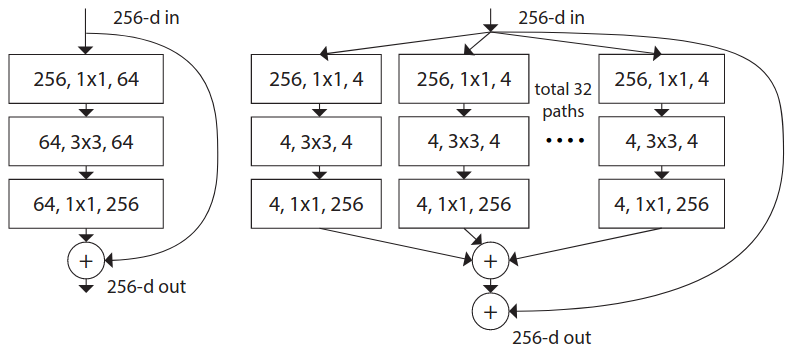
\includegraphics[width=1.0\textwidth]{figures/resnext-cardinality.png}
  \end{center}
  \caption{\textbf{Left}: A block of ResNet. \textbf{Right}: A block of ResNeXt with cardinality = 32. ~\cite{DBLP:journals/corr/XieGDTH16}}
  \label{fig:cardinality}
\end{figure}

\begin{figure}[H]
  \begin{center}
    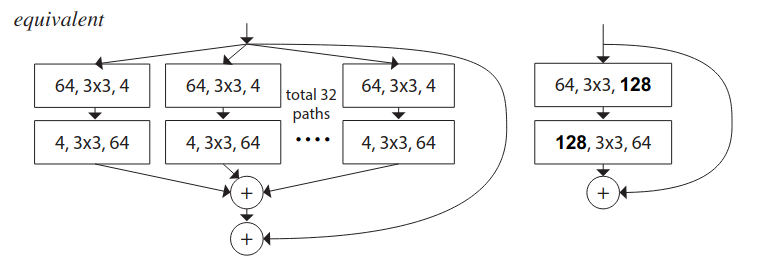
\includegraphics[width=1.0\textwidth]{figures/resnext-depth.png}
  \end{center}
  \caption{\textbf{Left}: Aggregating transformations of depth = 2 \textbf{Right}: An equivalent block, which is trivially wider.~\cite{DBLP:journals/corr/XieGDTH16}}
  \label{fig:depth}
\end{figure}



\subsubsection{Preprocessing}

Before training and inference, data augmentation is done to improve performance of the model or to make the model converge faster. The following steps are taken to augment the data:

\begin{enumerate}
\item Loading annotations (if training)
\item Image normalization
\item Image resizing
\item Random flipping
\item Padding
\item Image to tensor
\end{enumerate}

\textbf{Image normalization} normalizes the images by subtracting the mean and dividing by the inverse of the standard deviation of the RGB values of the dataset from the color channels.
When using pre-trained models it is advised to use the image normalization values for the dataset that the weights were acquired from.

\textbf{Image resizing} resizes the images' width and height to a random value in a fixed interval specified in the code. Annotation coordinates are scaled accordingly.

\textbf{Random flipping} flips the images horizontally at a rate of 50\%. Annotation coordinates are flipped accordingly.

\textbf{Padding} pads the images to a width and height divisible by 32.
Padding is done on the right and bottom side of the image, requiring no update to the coordinate of the masks and bounding boxes.
Padding is required when using FPNs to ensure that the feature maps align correctly when merged in a later stage of the network, unless all the input images can be assumed to have dimensions divisible by 32.

\textbf{Image to tensor} converts the resulting input into a \textit{tensor}.
A tensor is a data structure used to feed input to a neural network, and can contain more than one data point when using batches.


\subsection{Modifications to the primary architecture}

\textbf{Preprocessing}. Text embeddings are added to the data during the preprocessing step.
Because we want to avoid image normalization of the textual embeddings, and other preprocessing methods used by Mask R-CNN to augment the image data,
the textual embeddings are added as the last step. By the time we add the textual embeddings, the image may have been resized, padded and flipped horizontally.
The bounding boxes of the text embeddings are offset and scaled accordingly to align with the new dimensions.

\textbf{Classes}. Separate annotation files were generated to produce annotations for testing class confusion.
All values are identical except for the class id and names, which are all set to 'Publication unit'.
To conduct these experiments, the configuration files were duplicated and adjusted where classes were declared.

\textbf{Evaluation}. In the original MS COCO dataset (on which Mask R-CNN is usually evaluated),
there is size partitioning depending on the size of the object being detected when presented in the results.
Since the classes found in this project are generally larger on average than the size of the objects found in the MS COCO dataset,
the partitioning size thresholds are adjusted for these results to provide more useful information about different objects being detected (Using the standard thresholds, almost all objects are considered “large”).
This alteration has no impact on the performance of the solution itself, but must be considered when evaluating the results.

\begin{table}[H]
  \begin{center}
    \caption{Object size threshold differences in pixels}
    \label{tab:objectsizes}
    \begin{tabular}{l|l|l|l} % <-- Alignments: 1st column left, 2nd middle, with vertical lines in between
    \textbf{Dataset} & \textbf{Small} & \textbf{Medium} & \textbf{Large}  \\
    \hline
    MS COCO dataset & area < $32^2$ & $32^2$ < area < $96^2$ & area > $96^2$  \\    \hline
    This thesis & area < $283^2$ & $283^2$ < area < $600^2$ & area > $600^2$ \\    \hline
    \end{tabular}
  \end{center}
\end{table}

\begin{table}[H]
  \begin{center}
    \caption{Number of annotations per area group for the test sets}
    \label{tab:annotationspertestset}
    \begin{tabular}{l|l|l|l} % <-- Alignments: 1st column left, 2nd middle, with vertical lines in between
    \textbf{Area group} & \textbf{In-set} & \textbf{Near-set} & \textbf{Out-set}  \\
    \hline
    Small & 275 & 1207 & 825  \\    \hline
    Medium & 186 & 480 & 314 \\    \hline
    Large & 106 & 173 & 203 \\    \hline
    Total & 567 & 1860 & 1342 \\    \hline
    \end{tabular}
  \end{center}
\end{table}


\begin{figure}[H]
  \begin{center}
    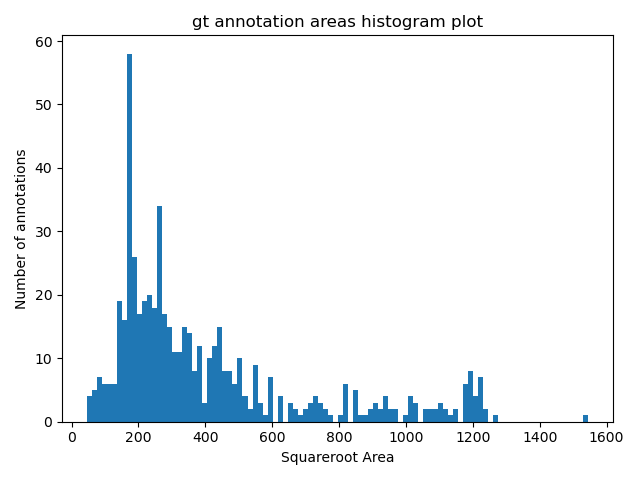
\includegraphics[width=0.6\textwidth]{figures/annotation-histogram-inset.png}
  \end{center}
  \caption{Distribution of annotations by squareroot area: Test subset of the DN 2010 - 2020 (In-set)}
  \label{fig:size_dist_annotations_in}
\end{figure}

\begin{figure}[H]
  \begin{center}
    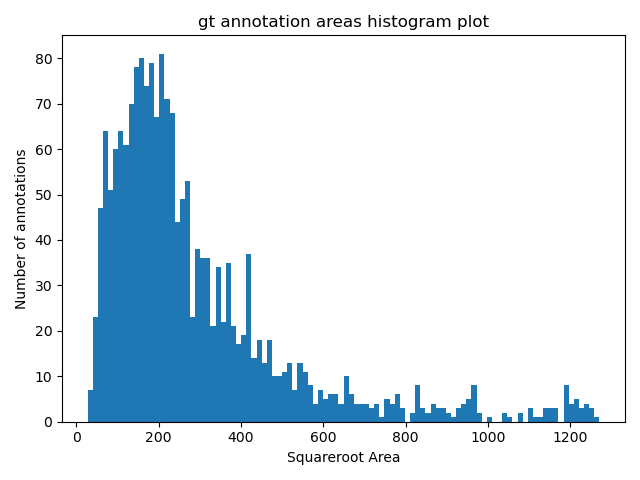
\includegraphics[width=0.6\textwidth]{figures/annotation-histogram-nearset.png}
  \end{center}
  \caption{Distribution of annotations by squareroot area: DN SvD 2001 - 2004 (Near-set)}
  \label{fig:size_dist_annotations_near}
\end{figure}

\begin{figure}[H]
  \begin{center}
    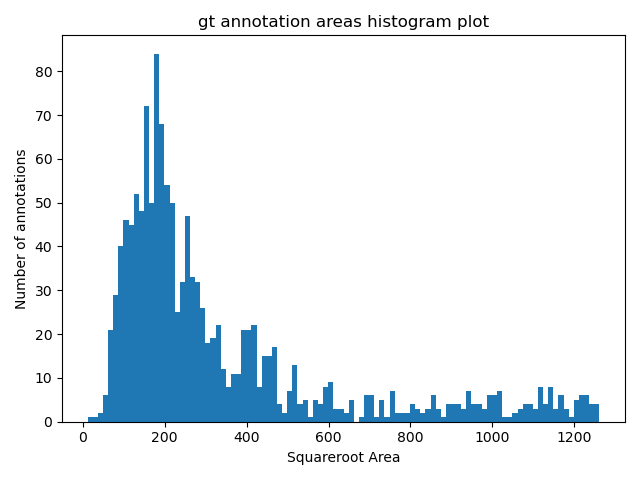
\includegraphics[width=0.6\textwidth]{figures/annotation-histogram-outset.png}
  \end{center}
  \caption{Distribution of annotations by squareroot area: Aftonbladet Expressen 2001 - 2004 (Out-set)}
  \label{fig:size_dist_annotations_out}
\end{figure}

\subsubsection{Multiscale training}

All models used in this thesis were trained using multiscale training. When using multiscale training in MMdetection, the training dataset can be repeated a number of times during training. When specifying the dimensions for the resizing operation in the preprocessing pipeline, the values are submitted as a range instead of fixed values which is the case for non-multiscale training. During training, a random width and height are generated from the ranges submitted in the configration. 

For the models that were altered to use text embeddings, the training dataset was not repeated due to insufficient memory. This was compensated for by increasing the number of epochs to 3 times that of other models. Consequently, the evaluation interval was increased from 1 to 3 to have an equal number of evaluation steps for all models. For all models not using text embeddings, the default value was used to repeat the training dataset during training, which is 3.

\subsubsection{Optimizer}

In the Mask R-CNN paper, the training is done on 8 GPUs, where each GPU processes 2 samples at a time (effective mini-batch size of 16) for a total of 280k iterations.
In this thesis, models were only trained using 1 GPU.

Stochastic gradient descent is used, with a learning rate is set to $0.02$ (for the first 160k iterations, which is decreased by 10 for the remaining 120k), a weight decay of $0.0001$, and momentum set to $0.9$.

Since we use only 1 GPU for training, according to the Linear Scaling Rule~\cite{DBLP:journals/corr/GoyalDGNWKTJH17}, we acquire a learning rate of $0.02/8=0.0025$.

A linear learning rate configuration was used. The learning rate was divided by 5 every 8th epoch for models without text embeddings, and every 24th epoch for models with text embeddings (resulting in the same number of iterations before every divide).

\subsection{Text Embedding map}

In order to combine the visual and textual information as input to the model, we map the one-dimensional representation of textual information (e.g. a word vector or paragraph vector) into a three-dimensional representation by positioning the embedding representation into a two-dimensional space (e.g. a word or paragraph has a certain width, height, x-, and y-coordinate of the top left corner when printed on a page).

This new textual embedding vector, corresponding to a character, word or paragraph, is equivalent to the original vector, augmented with the positional information. We refer to this three-dimensional representation of textual information, as mentioned in Barman et al~\cite{jdmdh:7097} and introduced in Yang et al.~\cite{DBLP:journals/corr/YangYAKKG17} as a ‘text embedding map’.

Notably, the key difference from the earlier works by Barman et al~\cite{jdmdh:7097} and Yang et al~\cite{DBLP:journals/corr/YangYAKKG17} is that in this approach the text embedding maps are generated on a paragraph level, instead of character- or word level.

The three-dimensional encoding of textual information is produced by using the result of an OCR process which outputs coordinates of bounding boxes for blocks of text together with its textual content.

We define this process formally as follows. Given an image of size $H$ $x$ $W$ and a list of tokens $T$ where each token $t$ is associated with a bounding box $b_t$ on the image, a text embedding map $G$ of size $H$ $x$ $W$ $x$ $N$ is produced, where $N$ is the dimension of the embeddings. Specifically, all pixels contained in the bounding box of a token $t$ are defined as the set $b_t \in {\rm I\!R}^2$ and each pixel $g_{i,j} \in G$ of the text embedding map is computed with

\begin{equation}
	g_{ij} =
	    \begin{cases}
	      E(t), & \text{if}\ (i,j) \in b_t \\
	      0^N, & \text{otherwise}
	    \end{cases}
  	\label{eqn:textembedding}
\end{equation}

where $E(t)$ is a mapping of $t \rightarrow {\rm I\!R}^N$ corresponding for example to a paragraph embedding, and $0^N$ is a null vector in case there is no text in the corresponding pixel. Each pixel overlapping with a bounding box produced by the OCR process is therefore mapped to its corresponding embedding. In this project, no bounding boxes are overlapping, which means no statement will be made regarding a strategy for such a case.

The result is a text embedding map, i.e. a three-dimensional matrix where the first two dimensions correspond to the image-localized representation of the text, and the third to the embedding itself. Given that the resulting matrix has the same width and height as the original image, it lends itself to easily extend the image input layer to accept more than its 3 original channels (RGB), that is to also fit an N-dimensional vector behind each pixel in a preprocessing step. The final number of channels of the input layer is therefore $3+N$, where the first 3 dimensions of each pixel contain the original RGB values of the input image.

\textbf{TODO Maybe visualization of the embedding maps?}

\subsubsection{Text embedding strategy}
\label{subs:textembeddingstrat}
There are a number of ways to embed the text behind the image channels in the final input.

\textbf{Text granularity}. As seen in \autoref{subs:dlapproaches}, there are options for encoding the text at different levels. There are binary masks, encoded vectors at word level, sentence level and paragraph level. When deciding to encode at word or sentence level, a strategy can be used to summarize the vectors across the entire text block if the exact coordiantes for the words or sentences cannot be attained. Alternatively, a strategy could be made to divide the text block into sections for each sentence within the block. 

In this thesis we transform the entire content of the text block and repeat the vector produced across the dimensions of the text block. 

\textbf{Text embedding normalization}. \textbf{TODO implement and compare}.

\textbf{Text embedding per sentence, divided equally on the text block}. \textbf{TODO implement and compare}.


\subsubsection{Sentence transformers}

We evaluate six different sentence transformers. Two are produced by the National Library of Sweden~\cite{swedish-bert} and output vectors of size 768. Four are created by Reimers et al~\cite{reimers-2019-sentence-bert, reimers-2020-multilingual-sentence-bert} and output vectors of size 384. These were selected by the performance on encoding sentences over 14 diverse tasks from different domains. 

\begin{table}[H]
  \begin{center}
    \caption{Sentence transformers}
    \label{tab:modeldimensions}
    \begin{tabular}{l|l}
    \textbf{Model name} & \textbf{Dimensions}  \\
    \hline
    all-mpnet-base-v2~\cite{reimers-2019-sentence-bert, reimers-2020-multilingual-sentence-bert} & 384 \\    \hline
    all-MiniLM-L6-v2~\cite{reimers-2019-sentence-bert, reimers-2020-multilingual-sentence-bert} & 384 \\    \hline
    multi-qa-mpnet-base-dot-v1~\cite{reimers-2019-sentence-bert, reimers-2020-multilingual-sentence-bert} & 384 \\    \hline
    all-distilroberta-v1~\cite{reimers-2019-sentence-bert, reimers-2020-multilingual-sentence-bert} & 384 \\    \hline
    KBLab/sentence-bert-swedish-cased~\cite{swedish-bert} & 768 \\    \hline
    KB/bert-base-swedish-cased~\cite{swedish-bert} & 768 \\    \hline
    \end{tabular}
  \end{center}
\end{table}

\clearpage

\section{Experiments}
\label{sec:experiments}

In this section we will introduce the experiments that will be conducted in order to attempt to achieve the goals outlined in \autoref{sec:goals}.

Because we labeled classes in the dataset creation process, we conduct an experiment to understand the impact of these classes on the model performance.

As mentioned in \autoref{subs:maskrcnn}, Mask R-CNN performs worse on smaller objects. An experiment will be conducted to investigate if we can exploit the large image sizes in our dataset to improve performance.


\subsection{Unimodal versus multimodal input}

One part of this thesis investigates the efficacy to one method of incorporating the textual modality into the model.
Baseline will be the unaltered Mask R-CNN models as they are implemented in framework we are using.

\subsection{Impact of class labels}

For the dataset created in this thesis, a number of classes are defined.
To investigate how these classes may impact performance, we conduct an experiment where all classes are converted to the same class.
In the comparison we will make, all other settings and parameters are equal.

\subsection{Impact of dataset size}

At the request of the researchers at the laboratory of the National Library of Sweden, we conduct an experiment to investigate if the model could potentially improve if a larger dataset was labeled. To investigate this matter, we create subsets of the training dataset at ratios of $0.25$, $0.5$, $0.75$ and $0.9$ and compare the results to the full training dataset size. All subsets were sampled using random sampling.

\begin{table}[H]
    \caption{Class distribution in partial datasets of DN 2010 - 2020 (In-set)}
    \label{tab:partialdist}
    \begin{tabular}{l|l|l|l|l|l|l} % <-- Alignments: 1st column left, 2nd middle, with vertical lines in between
    \textbf{\% Train} & \textbf{News Unit} & \textbf{Advertisement} & \textbf{Listing} & \textbf{Death Notice} & \textbf{Game} & \textbf{Weather}  \\
    \hline
    25\% & 212 & 149 & 225 & 23 & 18 & 2 \\    \hline
    50\% & 449 & 332 & 456 & 75 & 26 & 4 \\    \hline
    75\% & 648 & 500 & 618 & 66 & 36 & 11 \\    \hline
    90\% & 953 & 502 & 810 & 63 & 41 & 11 \\    \hline
    100\% & 1027 & 554 & 920 & 105 & 55 & 12 \\    \hline
    \end{tabular}
\end{table}


\subsection{Impact of image scaling}

In Mask R-CNN, two preprocessing pipelines are defined. One for data augmentation in the training process, and another for the evaluation step.

Preprocessing by data augmentation is common in deep learning in order to increase performance of the model.

One of these data augmentation steps resizes the input images to a range between $1333$ by $640$ pixels and $1333$ by $800$ pixels in the training phase. For evaluation, the images are resized to $1333$ by $800$ pixels.

As the images we have labeled in this thesis are larger than the images this model is usually trained and evaluated on,
we conduct an experiment where we scale these baseline values ($1333$, $640$, $800$) by a factor $0.5$, $1$, $2$, and $4$ to investigate model performance on this specific dataset.

By training and evaluating models with the same parameters while only varying the scaling factor mentioned previously, the impact can be investigated by comparing the performance of the models.


\section{Metrics}

\subsection{Mean Intersection over Union}

The Intersection over Union (IoU) is the standard metrics for semantic image segmentation and measures how well two sets of pixels are aligned. This is used to measure how much the boundary predicted by the algorithm overlaps with the ground truth (the real object boundary). Traditionally, with state-of-the-art datasets, an IoU threshold equal or greater to 0.5 is used to classify whether the prediction is a true positive or a false positive.

\begin{equation}
	IoU = \frac{Area \: Overlap}{Area \: Union}
  	\label{eqn:iou}
\end{equation}

The mean Intersection over Union(mIoU)~\cite{DBLP:journals/corr/LongSD14} is the IoU averaged over all classes to provide a global, mean IoU score. It is formulated as follows:

\begin{equation}
	Pixel \: accuracy = \frac{\sum_{i} n_{ii}}{\sum_{i}t_i}
  	\label{eqn:pixelacc}
\end{equation}

\begin{equation}
	Mean \: accuracy = \frac{1}{n_C} \sum_{i} n_{ii} / t_i
  	\label{eqn:meanacc}
\end{equation}

\begin{equation}
	mIoU = \frac{1}{n_C} \frac{\sum_{i} n_{ii}}{t_i + \sum_{i} n_{ji} - n_{ii}}
  	\label{eqn:meanIoU}
\end{equation}

where $n_{ij}$ is the number of pixels of class $i$ predicted to belong to class $j$, where there are $n_{C}$ different classes, and $t = \sum_{j} n_{ij}$ is the total number of pixels of class $i$.

\subsection{Precision and Recall}

The IoU does not quantify performances in terms of True Positives (TP), True Negatives (TN), False Positives (FP) and False Negatives (FN)~\cite{davis2006relationship}. These values are relevant when considering whether a model can be useful for real world applications, that is, if most of the segments are correctly recognized.

The standard way to measure these values in the field of segmentation is to consider a prediction as positive when above a certain threshold $\tau \in [0,1]$ of IoU. If the prediction is above the threshold $\tau$, it is well enough aligned with the ground truth and to be considered correct.

Given this definition, we can now consider:
\begin{enumerate}
\item A prediction with IoU $\geq \tau$ as True Positive(TP)
\item A prediction with no IoU (i.e. with a union of zero) as True Negative(TN)
\item A prediction with an IoU of zero and no predicted pixels (i.e. intersection of zero and non-zero number of pixels in the ground truth) as False Negative(FN)
\item A non-FN prediction with an IoU $< \tau$ as False Positive(FP)
\end{enumerate}

Given a threshold $\tau$, precision and recall are computed as follows:

\begin{equation}
	Precision @ \tau = P@\tau = \frac{TP}{(TP + FP)}
  	\label{eqn:precision}
\end{equation}

\begin{equation}
	Recall @ \tau = R@\tau = \frac{TP}{(TP + FN)}
  	\label{eqn:recall}
\end{equation}

It is also possible to compute the average precision and recall over a range of thresholds. This is defined by a start $\tau_{start}$, an end $\tau_{end}$, and a step size between two threshold $\tau_{step}$ using the following notation: $\tau_{start}$:$\tau_{step}$:$\tau_{end}$. Given a threshold range, the average metric $M$ (Where $M$ could be for example precision or recall) is then computed as follows:

\begin{equation}
M@\tau_{start}:\tau_{step}:\tau_{end} = \frac{1}{(\tau_{start}:\tau_{step}:\tau_{end})} \sum{} \tau \in \tau_{start}:\tau_{step}:\tau_{end}
    \label{eqn:rangem}
\end{equation}

It should be noted that metrics such as IoU, mIoU, Precision and Recall are computed at the page level and not at the instance level. If a page contains several instances of a class and the prediction only matches some instances, thus not enough to reach an IoU threshold larger than $\tau$, the whole page is counted as negative.


\subsection{Mean Average Precision}

The mean Average Precision (mAP)~\cite{zhang2009average} was used to evaluate detection performance. The mAP metric is the product of precision and recall of detected bounding boxes. The mAP value ranges from 0 to 1, with higher values being better. The mAP can be computed by calculating average precision (AP) separately for each class (including background) and then averaging over the classes. A detection is considered a true positive only if the IoU is above a certain threshold.

All detections from test images may be combined in a precision/recall curve. The final area under the curve is used to compare the algorithms. If $N$ represents the number of images, the mAP can be computed as follows:

\begin{equation}
mAP = \frac{1}{N} \sum_{i=1}^{N} AP_i
    \label{eqn:map}
\end{equation}


\chapter{Results}
\label{ch:results}

In this section we present the results of the neural network architectures for the datasets created in this thesis. Naming convention follows the original Mask R-CNN paper and results are presented by bounding box ($bb$) and segmentation mask ($m$) respectively, as it is presented in the Mask R-CNN paper.

\section{Unimodal versus multimodal}

\begin{table}[H]
  \begin{center}
    \caption{Model names}
    \label{tab:modelnames}
    \resizebox{\columnwidth}{!}{
    \begin{tabular}{l|l|l|l|p{1.5cm}}
    \textbf{Final name} & \textbf{Head} & \textbf{Backbone} & \textbf{Sentence transformer} & \textbf{Text embeddings length} \\
    \hline
    r50-FPN-vanilla & resnet50 & FPN & None & 0 \\    \hline
    x101-32x8d-FPN-vanilla & resnext101 & FPN & None & 0 \\    \hline
    x101-64x4d-FPN-vanilla & resnext101 & FPN & None & 0 \\     \hline
    More & models & in & final & paper \\     \hline
    r50-FPN-KBLab & resnext101 & FPN & KBLab/sentence-bert-swedish-cased & 768 \\     \hline
    r50-FPN-KB & resnet50 & FPN & KB/bert-base-swedish-cased & 768 \\     \hline
    \end{tabular}}
  \end{center}
\end{table}


\begin{table}[H]
  \begin{center}
    \caption{Results on the DN 2010 - 2020 (In-set) dataset}
    \label{tab:dn2010results}
    \resizebox{\columnwidth}{!}{
    \begin{tabular}{l|l|l|l|l|l|l} %
    \textbf{Final name} & \textbf{$mAP_m$} & \textbf{$mAP_m^{50}$} & \textbf{$mAP_m^{75}$} & \textbf{$mAP_{bb}$} & \textbf{$mAP_{bb}^{50}$} & \textbf{$mAP_{bb}^{75}$} \\
    \hline
    r50-FPN-vanilla & 0.0 & 0.0 & 0.0 & 0.0 & 0.0 & 0.0 \\    \hline
    x101-32x8d-FPN-vanilla & 0.0 & 0.0 & 0.0 & 0.0 & 0.0 & 0.0 \\    \hline
    x101-64x4d-FPN-vanilla & 0.0 & 0.0 & 0.0 & 0.0 & 0.0 & 0.0 \\     \hline
    \end{tabular}}
  \end{center}
\end{table}

\begin{table}[H]
  \begin{center}
    \caption{Results on the DN SvD 2001 - 2004 (Near-set) dataset}
    \label{tab:dnsvd2001results}
    \resizebox{\columnwidth}{!}{
    \begin{tabular}{l|l|l|l|l|l|l}
    \textbf{Final name} & \textbf{$mAP_m$} & \textbf{$mAP_m^{50}$} & \textbf{$mAP_m^{75}$} & \textbf{$mAP_{bb}$} & \textbf{$mAP_{bb}^{50}$} & \textbf{$mAP_{bb}^{75}$} \\
    \hline
    r50-FPN-vanilla & 0.0 & 0.0 & 0.0 & 0.0 & 0.0 & 0.0 \\    \hline
    x101-32x8d-FPN-vanilla & 0.0 & 0.0 & 0.0 & 0.0 & 0.0 & 0.0 \\    \hline
    x101-64x4d-FPN-vanilla & 0.0 & 0.0 & 0.0 & 0.0 & 0.0 & 0.0 \\     \hline
    \end{tabular}}
  \end{center}
\end{table}

\begin{table}[H]
  \begin{center}
    \caption{Results on the Aftonbladet Expressen 2001 - 2004 (Out-set) dataset}
    \label{tab:abexpresults}
    \resizebox{\columnwidth}{!}{
    \begin{tabular}{l|l|l|l|l|l|l}
    \textbf{Final name} & \textbf{$mAP_m$} & \textbf{$mAP_m^{50}$} & \textbf{$mAP_m^{75}$} & \textbf{$mAP_{bb}$} & \textbf{$mAP_{bb}^{50}$} & \textbf{$mAP_{bb}^{75}$} \\
    \hline
    r50-FPN-vanilla & 0.0 & 0.0 & 0.0 & 0.0 & 0.0 & 0.0 \\    \hline
    x101-32x8d-FPN-vanilla & 0.0 & 0.0 & 0.0 & 0.0 & 0.0 & 0.0 \\    \hline
    x101-64x4d-FPN-vanilla & 0.0 & 0.0 & 0.0 & 0.0 & 0.0 & 0.0 \\     \hline
    \end{tabular}}
  \end{center}
\end{table}

\section{Impact of class labels}

\textbf{TODO text and table here.}

\section{Impact of dataset size}

All results reported in this section are averaged over 5 runs. The standard deviation $\sigma$ denotes the average of the standard deviations of each column. 

\begin{table}[H]
  \begin{center}
    \caption{Gradually increasing dataset size - All classes - In set}
    \label{tab:dsizeallcinset}
    \resizebox{\columnwidth}{!}{
    \begin{tabular}{l|l|l|l|l|l|l|l}
    \textbf{\% Train} & \textbf{$mAP_m$} & \textbf{$mAP_m^{50}$} & \textbf{$mAP_m^{75}$} & \textbf{$mAP_{bb}$} & \textbf{$mAP_{bb}^{50}$} & \textbf{$mAP_{bb}^{75}$} & \textbf{$\sigma$} \\
    \hline
    25\% & 0.460 & 0.690 & 0.482 & 0.448 & 0.597 & 0.430 & 0 \\    \hline
    50\% & 0.747 & 0.832 & 0.790 & 0.713 & 0.832 & 0.789 & 0  \\    \hline
    75\% & 0.750 & 0.822 & 0.808 & 0.752 & 0.822 & 0.810 & 0  \\     \hline
    90\% & 0.595 & 0.664 & 0.620 & 0.592 & 0.665 & 0.617 & 0 \\     \hline
    100\% & 0.851 & 0.944 & 0.875 & 0.842 & 0.943 & 0.878 & 0  \\     \hline
    \end{tabular}}
  \end{center}
\end{table}

\begin{table}[H]
  \begin{center}
    \caption{Gradually increasing dataset size - All classes - Near set}
    \label{tab:dsizeallcnearset}
    \resizebox{\columnwidth}{!}{
    \begin{tabular}{l|l|l|l|l|l|l|l}
    \textbf{\% Train} & \textbf{$mAP_m$} & \textbf{$mAP_m^{50}$} & \textbf{$mAP_m^{75}$} & \textbf{$mAP_{bb}$} & \textbf{$mAP_{bb}^{50}$} & \textbf{$mAP_{bb}^{75}$} & \textbf{$\sigma$} \\
    \hline
    25\% & 0.220 & 0.309 & 0.219 & 0.210 & 0.309 & 0.218 & 0 \\    \hline
    50\% & 0.376 & 0.459 & 0.378 & 0.365 & 0.457 & 0.374 & 0  \\    \hline
    75\% & 0.343 & 0.409 & 0.366 & 0.336 & 0.409 & 0.361 & 0 \\     \hline
    90\% & 0.275 & 0.350 & 0.287 & 0.267 & 0.352 & 0.290 & 0 \\     \hline
    100\% & 0.414 & 0.481 & 0.430 & 0.402 & 0.481 & 0.423 & 0  \\     \hline
    \end{tabular}}
  \end{center}
\end{table}

\begin{table}[H]
  \begin{center}
    \caption{Gradually increasing dataset size - All classes - Out set}
    \label{tab:dsizeallcoutset}
    \resizebox{\columnwidth}{!}{
    \begin{tabular}{l|l|l|l|l|l|l|l}
    \textbf{\% Train} & \textbf{$mAP_m$} & \textbf{$mAP_m^{50}$} & \textbf{$mAP_m^{75}$} & \textbf{$mAP_{bb}$} & \textbf{$mAP_{bb}^{50}$} & \textbf{$mAP_{bb}^{75}$} & \textbf{$\sigma$} \\
    \hline
    25\% & 0.389 & 0.476 & 0.423 & 0.377 & 0.474 & 0.413 & 0 \\    \hline
    50\% & 0.330 & 0.425 & 0.355 & 0.325 & 0.425 & 0.353 & 0  \\    \hline
    75\% & 0.288 & 0.368 & 0.310 & 0.282 & 0.368 & 0.310 & 0  \\     \hline
    90\% & 0.290 & 0.356 & 0.310 & 0.279 & 0.355 & 0.289 & 0 \\     \hline
    100\% & 0.488 & 0.599 & 0.527 & 0.451 & 0.598 & 0.461 & 0 \\    \hline
    \end{tabular}}
  \end{center}
\end{table}



\section{Impact of image scaling}

\textbf{TODO text and table here about results of image size augmentation.}


\chapter{Discussion}
\label{ch:disc}

\section{Mask R-CNN}

\subsection{Higher performance is required for usefulness within the domain of newspaper article segmentation}

Results reported on the performance of the Mask R-CNN architecture on the MS COCO dataset may seem less impressive for the metrics  \textbf{$mAP_m$} \textbf{$mAP_m^{50}$} \textbf{$mAP_m^{75}$} \textbf{$mAP_{bb}$} \textbf{$mAP_{bb}^{50}$} \textbf{$mAP_{bb}^{75}$}. These metrics are not directly comparable due to the lack of irregular shapes of news article content compared to "common objects in context". Mask R-CNN can however be said to be able to segment content based on multiple elements being seen as one instance of an object, which is essential to newspaper article segmentation.

\subsection{Unaltered Mask R-CNN performs well on in-domain datasets} 

The impressive results on the in-set indicate that the newspaper typology is learned well by the model, and the less impressive results on the near-set and out-set indicate that the generalization property is lacking purely from training on one typology and newspaper. Labeling a reasonable amount from each design era and newspaper respectively could give an overall well performing model.

\section{Classes}
By limiting the number of classes to one, the burden of determining the class becomes a boolean problem. It should be expected that this task yields greater performance, as this task is more trivial than additionally determining the specific subclass especially if the classes are constructed by subjective criteria or implication.

\section{Sentence transformers}

\subsection{Large text embeddings} 

As seen \autoref{tab:modeldimensions}, the sentence transformers output their vectors of size $768$ or $384$. This adds a significant number of channels to the input if inserted without alteration. The consequence is a large memory footprint. Additionally, using an otherwise unaltered Mask R-CNN architecture, this puts a lot of responsibility for layers closer to the input layer to discern the importance of the additional information.  

\subsection{Text granularity}

As mentioned in \autoref{subs:textembeddingstrat}, there are many ways to segment the blocks of text recognized by the OCR. Further work is needed to determine the most effective way to present this information as input to deep learning models.

\section{Combining other methods}

The models proposed in this thesis need not be used in an end-to-end fashion. Spatial information available through OCR could be used in conjunction with these models to improve determining element relatedness or other end uses. 

\chapter{Conclusions and Future Work}
\label{ch:conc}
\section{Conclusions}
\section{Limitations}


\section{Future work}

\begin{itemize}
\item \textbf{Pairwise merged newspaper pages.} Per newspaper page instance segmentation has its drawbacks. Newspapers are meant to be read mostly overviewing two pages simultaniously. "Implied content" could be avoided by merging pages pairwise before annotation.
\item \textbf{Domain-specific architecture.} Developing specific head and backbone architecture to incorporate the textual embeddings puts less reliance on the traditional head and backbone architectures to adapt to the new input medium.
\item \textbf{Dataset size}. Dataset size increases could potentially lead to more stable results and a greater diversity in topology and time-period could lead to a greater generalization property.
\item \textbf{Dimensionality reduction}. Principle Component Analysis (PCA) or any other dimensionality reduction algorithm could be used to compress the vector representation. This could be useful to limit the memory footprint of the input, and potentially denoise the input.
\item \textbf{Image normalization and training without pretrained weights}. In this thesis, image normalization values were left unchanged and training was done using the pretrained weights for the respective architectures. Could using dataset specific image normalization values and training models from scratch improve results?
\end{itemize}


%The thesis contributes to the \gls{UN}\enspace\glspl{SDG} numbers 1 and 9 by
%xxxx.

\noindent\rule{\textwidth}{0.4mm}

\cleardoublepage
% Print the bibliography (and make it appear in the table of contents)
\renewcommand{\bibname}{References}
\addcontentsline{toc}{chapter}{References}

\ifbiblatex
    %\typeout{Biblatex current language is \currentlang}
    \printbibliography[heading=bibintoc]
\else
    \bibliography{references}
\fi



\appendix
\renewcommand{\chaptermark}[1]{\markboth{Appendix \thechapter\relax:\thinspace\relax#1}{}}

\section{Appendix A: Definitions related to news articles}
\label{app:newsarticle}

\begin{definition}
\label{headline}
A \textbf{headline} is a very short summary of a news report. It normally appears in large letters above the report. [Cambridge Dictionary]
\end{definition}

\begin{definition}
\label{subhead}
A \textbf{subhead} or subheading is a word, phrase, or sentence that is used to introduce part of a text. [Cambridge Dictionary]
\end{definition}

\begin{definition}
\label{preamble}
A \textbf{preamble} is an introduction to a speech or piece of writing. [Cambridge Dictionary]
\end{definition}

\begin{definition}
\label{body text}
A \textbf{body text} is the main part of a printed text, excluding items such as headings and footnotes. [Oxford Languages]
\end{definition}

\begin{definition}
\label{byline}
A \textbf{byline} is a line at the top or bottom of a newspaper or magazine article giving the writer's name. [Cambridge Dictionary]
\end{definition}

\begin{definition}
\label{img}
An \textbf{image caption} or a \textbf{video caption} is a title or brief explanation accompanying an illustration, cartoon, poster or in the latter case a video. [Oxford Languages]
\end{definition}

%% The following label is necessary for computing the last page number of the body of the report to include in the "For DIVA" information
\label{pg:lastPageofMainmatter}

\clearpage
\fancyhead{}  % Do not use header on this extra page or pages
% TODO diva stuff
%\section*{For DIVA}
%\lstset{numbers=none} %% remove any list line numbering
%\divainfo{pg:lastPageofPreface}{pg:lastPageofMainmatter}
\end{document}
